% Options for packages loaded elsewhere
\PassOptionsToPackage{unicode}{hyperref}
\PassOptionsToPackage{hyphens}{url}
%
\documentclass[
]{article}
\usepackage{amsmath,amssymb}
\usepackage{lmodern}
\usepackage{iftex}
\ifPDFTeX
  \usepackage[T1]{fontenc}
  \usepackage[utf8]{inputenc}
  \usepackage{textcomp} % provide euro and other symbols
\else % if luatex or xetex
  \usepackage{unicode-math}
  \defaultfontfeatures{Scale=MatchLowercase}
  \defaultfontfeatures[\rmfamily]{Ligatures=TeX,Scale=1}
\fi
% Use upquote if available, for straight quotes in verbatim environments
\IfFileExists{upquote.sty}{\usepackage{upquote}}{}
\IfFileExists{microtype.sty}{% use microtype if available
  \usepackage[]{microtype}
  \UseMicrotypeSet[protrusion]{basicmath} % disable protrusion for tt fonts
}{}
\makeatletter
\@ifundefined{KOMAClassName}{% if non-KOMA class
  \IfFileExists{parskip.sty}{%
    \usepackage{parskip}
  }{% else
    \setlength{\parindent}{0pt}
    \setlength{\parskip}{6pt plus 2pt minus 1pt}}
}{% if KOMA class
  \KOMAoptions{parskip=half}}
\makeatother
\usepackage{xcolor}
\usepackage[margin=1in]{geometry}
\usepackage{graphicx}
\makeatletter
\def\maxwidth{\ifdim\Gin@nat@width>\linewidth\linewidth\else\Gin@nat@width\fi}
\def\maxheight{\ifdim\Gin@nat@height>\textheight\textheight\else\Gin@nat@height\fi}
\makeatother
% Scale images if necessary, so that they will not overflow the page
% margins by default, and it is still possible to overwrite the defaults
% using explicit options in \includegraphics[width, height, ...]{}
\setkeys{Gin}{width=\maxwidth,height=\maxheight,keepaspectratio}
% Set default figure placement to htbp
\makeatletter
\def\fps@figure{htbp}
\makeatother
\setlength{\emergencystretch}{3em} % prevent overfull lines
\providecommand{\tightlist}{%
  \setlength{\itemsep}{0pt}\setlength{\parskip}{0pt}}
\setcounter{secnumdepth}{-\maxdimen} % remove section numbering
\usepackage{booktabs}
\usepackage{longtable}
\usepackage{array}
\usepackage{multirow}
\usepackage{wrapfig}
\usepackage{float}
\usepackage{colortbl}
\usepackage{pdflscape}
\usepackage{tabu}
\usepackage{threeparttable}
\usepackage{threeparttablex}
\usepackage[normalem]{ulem}
\usepackage{makecell}
\usepackage{xcolor}
\usepackage{caption}
\ifLuaTeX
  \usepackage{selnolig}  % disable illegal ligatures
\fi
\IfFileExists{bookmark.sty}{\usepackage{bookmark}}{\usepackage{hyperref}}
\IfFileExists{xurl.sty}{\usepackage{xurl}}{} % add URL line breaks if available
\urlstyle{same} % disable monospaced font for URLs
\hypersetup{
  pdftitle={Toronto Neighbourhood Crime},
  hidelinks,
  pdfcreator={LaTeX via pandoc}}

\title{Toronto Neighbourhood Crime}
\usepackage{etoolbox}
\makeatletter
\providecommand{\subtitle}[1]{% add subtitle to \maketitle
  \apptocmd{\@title}{\par {\large #1 \par}}{}{}
}
\makeatother
\subtitle{Examining the relationship between Neighbourhood Crime Rate
and Demographic Data in Toronto's 140 historical neighbourhoods in 2016}
\author{}
\date{\vspace{-2.5em}24 April 2022}

\begin{document}
\maketitle

{
\setcounter{tocdepth}{2}
\tableofcontents
}
\hypertarget{introduction}{%
\section{1. Introduction}\label{introduction}}

This research study aims to explore the relationship between crime rate
and the characteristics of neighbourhoods in Toronto in 2016. Past
studies showed that neighbourhood characteristics were significant
factors of the crime rate of an area (Foster et.al 2010\footnote{Foster,
  S., Giles-Corti, B., \& Knuiman, M. (2010). Neighbourhood design and
  fear of crime: A social-ecological examination of the correlates of
  residents' fear in new suburban housing developments. In Health \&
  Place (Vol. 16, Issue 6, pp.~1156--1165). Elsevier BV.
  \url{https://doi.org/10.1016/j.healthplace.2010.07.007}}). These
characteristics include: social-economic factors such as number of
businesses, number of community spaces such as parks, green spaces and
community centers, ease of transit access, and human factors such as
community belonging and quality of local communities (Statistics Canada
2021\footnote{Statistics Canada. (2021). Neighbourhood characteristics
  and life satisfaction of individuals in lower-, middle-, and
  higher-income families in Canadian metropolitan areas. Government of
  Canada. \url{https://doi.org/10.25318/36280001202100500006-ENG}}). In
this study, we aim to explore the relationship between the demographics,
neighbourhood amenities and crime rate of neighbourhoods. Understanding
this relationship will help the government and local communities respond
more effectively against emerging crime rates, by eliminating risk
factors and improving the well-being of a neighbourhood.

From 1996 to 2021, the City of Toronto was divided into 140 (historical)
neighbourhoods. On 12 April 2022, Toronto's social planning
neighbourhoods changed which resulted in an increase of the number of
neighbourhoods to 158. This research used the historical neighbourhoods
planning, since all data were collected before 2022. The sources of data
used come from the following sources:
\href{https://www.toronto.ca/city-government/data-research-maps/open-data/}{the
City of Toronto's Open Data Portal},
\href{https://www.statcan.gc.ca/en/start}{Statistics Canada}, and
several custom datasets from \href{https://www.kaggle.com/}{Kaggle}.
Crime rates and police-reported crimes were collected from the first
source, while Statistics Canada provided census data via Census of
Population, containing information about people and housing units in
Canada by their demographics, social and economic
characteristics\footnote{Government of Canada, S. C. (2020, July 17).
  Census of population. Surveys and statistical programs. Retrieved
  March 13, 2023, from
  \url{https://www23.statcan.gc.ca/imdb/p2SV.pl?Function=getSurvey\&SDDS=3901}}.

We first identified main demographics factors which were thought to be
highly correlated with neighbourhood crime rates, by examining past
studies of similar research: crime rates were found to be lower in
neighbourhoods with higher proportions of senior citizens and
immigrants, and in neighbourhoods which were further away from the urban
city centers\footnote{Statistics Canada. (n.d.). Main article.
  Neighbourhood Characteristics and the Distribution of Police-reported
  Crime in the City of Toronto. Retrieved March 13, 2023, from
  \url{https://www150.statcan.gc.ca/n1/pub/85-561-m/2009018/part-partie1-eng.htm}};
the proportion of visible minorities and racial heterogeneity were also
found to be correlated to neighbourhood crime rates\footnote{Sun, Ivan
  Y.; Triplett, Ruth A.; and Gainey, Randy R., ``Neighborhood
  Characteristics and Crime: A Test of Sampson and Groves' Model of
  Social Disorganization'' (2004). Sociology \& Criminal Justice Faculty
  Publications. 3.
  \url{https://digitalcommons.odu.edu/sociology_criminaljustice_fac_pubs/3}}.

In terms of social-economic factors such as community amenities and
businesses of the neighbourhood, commercial activities were found to be
correlated with higher crime rate, but this relationship was mostly due
to the dining businesses which opened after midnight\footnote{Twinam, T.
  (2017, May 25). Danger zone: Land use and the geography of
  neighborhood crime. Retrieved April 25, 2023, from
  \url{https://www.sciencedirect.com/science/article/abs/pii/S009411901730044X?dgcid=raven_sd_aip_email}}.
On the other hand, researchers discovered that short-term housing, such
as Airbnb rentals, contributed to higher crime rate in the surrounding
area, although the increase in crime often happened after a year or more
following an increase in rental listings\footnote{Ke, L., O'Brien, D.
  T., \& Heydari, B. (2021, July 14). Airbnb and neighborhood crime: The
  incursion of tourists or the erosion of local social dynamics? PLOS
  ONE. Retrieved April 25, 2023, from
  \url{https://journals.plos.org/plosone/article?id=10.1371\%2Fjournal.pone.0253315}}.

These studies provided preliminary insights for us to select the
important variables and observations from thousands of features in the
census data, as well as retrieving representative data from other
sources.

This report outlines the process of data collection, exploratory data
analysis and preliminary testing, modeling, interpreting results and
findings.

\hypertarget{methods}{%
\section{2. Methods}\label{methods}}

\hypertarget{data-collection}{%
\subsection{2.1 Data Collection}\label{data-collection}}

To answer our research question, data were collected from The City of
Toronto's Open Data Portal (the Portal), the official source for Toronto
open data from city divisions and agencies\footnote{\url{https://open.toronto.ca/}}.
The datasets of interest were ``Major Crime Indicators'' and
``Neighbourhood Profiles''. Both datasets were readily available for
download on Open Toronto as a CSV, JSON or XML format, or by using the
Open Data Portal API. We retrieved the data by downloading the CSV
file\footnote{We originally retrieved the data through the portal's API,
  by installing the R package opendatatoronto and following the
  instructions in the ``For Developers'' section (See
  \href{https://open.toronto.ca/dataset/neighbourhood-profiles/}{Neighbourhood
  Profiles} and
  \href{https://open.toronto.ca/dataset/major-crime-indicators/}{Major
  Crime Indicators}. However, the Portal updated their API and the
  format of the data (i.e.~the column names), which rendered our old
  code unusable.}. The ``Neighbourhoods'' dataset was also retrieved as
a geojson file from the Portal for creating a map visualization of crime
rate: it contained the coordinates of the boundaries of the 140
historical neighbourhoods in Toronto. Lastly, two datasets were used
from Kaggle,
\href{https://www.kaggle.com/datasets/suchow32/airbnb-toronto-data}{Airbnb
Toronto Data} and
\href{https://www.kaggle.com/datasets/youssef19/toronto-neighborhoods-inforamtion}{Toronto
Neighborhoods Information}. As their names suggest, the former provide
listings of Airbnb rentals in Toronto and the latter used the Foursquare
API (among others) to provide additional information about Toronto
neighbourhoods.

\hypertarget{dataset---major-crime-indicators}{%
\subsubsection{2.1.1 Dataset - Major Crime
Indicators}\label{dataset---major-crime-indicators}}

This dataset contains all Major Crime Indicators (MCIs) occurrences in
140 historical neighbourhoods in Toronto with reported date in between 1
January 2014 and 30 June 2022. The MCIs are divided into five
categories: Assault, Break and Enter, Auto Theft, Robbery and Theft
Over. The Indicators excludes the Sexual Violation offences.

The variables of interest include the MCI category (mci\_category), the
offence (Offence), the neighbourhood of occurrence (Neighbourhood), and
the occurrence and reported date and time. According to the dataset
description, the data is provided at the offence and/or victim level,
thus one occurrence of a crime major appear several times, each
associated with different MCI categories; that is, an offence could be
categorized into several categories and reported multiple times in the
data\footnote{\url{https://open.toronto.ca/dataset/major-crime-indicators/}}.

Table 1 in the Appendix shows the top four rows of the raw data.
Descriptions of the variables can be found in the
\href{https://torontops.maps.arcgis.com/sharing/rest/content/items/c0b17f1888544078bf650f3b8b04d35d/data}{Public
Safety Data Portal: Open Data Documentation}, or in the ``Data
Cleaning'' section below.

\hypertarget{dataset---neighbourhood-profiles}{%
\subsubsection{2.1.2 Dataset - Neighbourhood
Profiles}\label{dataset---neighbourhood-profiles}}

This dataset includes census data of the 140 neighbourhoods in the City
of Toronto in 2016. It contains over 2300 features of the
neighbourhoods, spanning areas such as population, language, income,
housing, education, and labour. There are over 2300 rows in the dataset,
each representing a characteristic (feature) among the 50 topics,
including marital status, income of individuals etc. Each characteristic
has several sub-characteristics, for example, for the income response,
there were different levels of income (\$10000-\$14999, \$15000-\$19999
etc.). Based on our findings on prior research on crime rate, these were
the demographic characteristics of interest: age, level of education,
employment status, immigration and citizenship status, average income
tax, number of visible minorities, and population count.

The data were originally collected through the Census of Population
conducted nationwide by Statistical Canada, which did not release the
complete data at the level of individual neighbourhoods. However, it was
aggregated by Toronto Open Data into the levels of neighbourhood and the
result was summarized in this dataset. Nonetheless, a small amount of
data released in the Census could not be aggregated to the levels of
neighbourhoods, such as summaries of income distribution of residents in
the City of Toronto as a whole. This did not deter our study as the
amount of data not released at the level of neighbourhoods were
significantly less than not, and the variables we chose were not any of
affected variables.

Note that Statistics Canada carry out random rounding reporting
practices, which may have an effect on aggregated statistics such as
median, percentages and mean of groups with low number of
observations\footnote{\url{https://open.toronto.ca/dataset/neighbourhood-profiles/}}.

Table 2 in the Appendix below shows the top four rows of the raw data.
Descriptions of the variables can be found in the
\href{https://torontops.maps.arcgis.com/sharing/rest/content/items/c0b17f1888544078bf650f3b8b04d35d/data}{Public
Safety Data Portal: Open Data Documentation}, or in the ``Data
Cleaning'' section below.

\hypertarget{dataset---airbnb-toronto-data}{%
\subsubsection{2.1.3 Dataset - Airbnb Toronto
Data}\label{dataset---airbnb-toronto-data}}

This dataset from Kaggle contains over 16000 observations of Airbnb
rental listings in Toronto on 4th November 2022. The author collected
the data through the \href{http://insideairbnb.com/get-the-data/}{Inside
Airbnb} website, which provides quarterly data of Airbnb listings in
cities around the world. The dataset was then cleaned by the author such
that each listing was located in one of the 140 historical
neighbourhoods of Toronto. The variables include the listing's owner,
neighbourhood, the price, property and room type etcetera.

Although the dataset was collected in 2022, it still provided invaluable
insights of the distribution of short term rentals in the city of
Toronto, assuming that each region has roughly the same changes in the
number of listings over the years. Note that data from previous years
were available at a price.

\hypertarget{dataset---toronto-neighbourhood-information}{%
\subsubsection{2.1.4 Dataset - Toronto Neighbourhood
Information}\label{dataset---toronto-neighbourhood-information}}

Similar to our other data sources, the Kaggle author created this
dataset in March 2021 by combining data from ``Neighbourhood Profiles'',
``Neighbourhood Crime Rates'' from Statistical Canada, and venue
information from Foursquare API . The data extracted from the first two
sources were heavily cleaned and preprocessed, which did not matter
because we already obtained the original datasets from the official
sources (as stated above). The only data we were interested in was the
gym and venue information data from Foursquare API, which contained the
number of gyms and points of interest in each neighbourhood.

Although this dataset was collected after 2016, it was still important
to our research as the number of venues and points of interests should
roughly remain the same throughout these years.

\hypertarget{data-cleaning-and-wrangling}{%
\subsection{2.2 Data Cleaning and
Wrangling}\label{data-cleaning-and-wrangling}}

For all the datasets, we first inspected the datasets using R functions
such as summary, str, dim, head, is.na and functions from the tidyverse
package to group and filter the data to better understand the
characteristics of the data by different groups.

\hypertarget{cleaning-of-major-crime-indicators}{%
\subsubsection{2.2.1 Cleaning of ``Major Crime
Indicators''}\label{cleaning-of-major-crime-indicators}}

Unwanted variables were first removed. They included: X\_id (unique
identifier), event\_unique\_id (event identifier), Division (Police
Division where offence occurred), ucr\_code (UCR code for offence),
ucr\_ext (UCR extension for offence), and Hood\_ID (identifier of
neighbourhood).

The remaining wanted variables contained information about the
occurrence time and date (in variables occurrencedate, occurrenceyear,
occurrencemonth, occurrenceday, occurrencedayofyear,
occurrencedayofweek, occurrencehour), the reported time and date (in
variables reporteddate, reportedyear, reportedmonth, reportedday,
reporteddayofyear, reporteddayofweek, reportedhour), the location (in
variables location\_type, premises\_type, Neighbourhood), and the crime
offence (in variables Offence and MCI).

Observations not from 2016 were also removed, since we were only
interested in reported offences which occurred in 2016. We also removed
observations where the neighbourhood was missing, which was represented
by ``NSA'' (``Not Specified Area'') in the data.

\hypertarget{cleaning-of-neighbourhood-profiles}{%
\subsubsection{2.2.2 Cleaning of ``Neighbourhood
Profiles''}\label{cleaning-of-neighbourhood-profiles}}

The ``Neighbourhood Profiles'' dataset contains characteristics
(features) which have sub-characteristics (sub-features). However, these
sub-characteristics are all listed under the same column (same variable)
as the parent characteristic, except being indented by varying degrees
based on the sub-characteristic relationships (i.e.~a
sub-sub-characteristic is indented more than a sub-characteristics, and
so on). Moreover, some of the rows in the data are in complete wrong
order, which made data cleaning inefficient and prone to error. For
example, two sub-characteristics with very similar description are
placed in the same indentation under the two characteristics of similar
type (in the wrong order), which makes it impossible to distinguish
which sub-characteristics belongs to which parent. To tackle this
problem, we first identified the main characteristics wanted before
cleaning the sub-characteristics.

We first removed the ``Data Source'' column (which defines the data
source, unrelated to our research) and divided the dataset into 50
tibbles, each representing a different topic with varying number of
(sub-)characteristics. Then, we cleaned only the features
(characteristics) wanted: age, level of education, employment status,
immigration and citizenship status, average income tax, number of
visible minorities, and population count. These features were kept in
separate tables for the purpose of preliminary testing individually.
Note that some of these subtables still suffered from faulty
arrangements and we could only use a subset of these sub-tables in our
study.

\hypertarget{cleaning-of-airbnb-toronto-data}{%
\subsubsection{2.2.3 Cleaning of ``Airbnb Toronto
Data''}\label{cleaning-of-airbnb-toronto-data}}

The dataset was already cleaned by the maker. However, although the
variable is named neighbourhood\_cleansed, some neighbourhood names were
not standardized. Thus, we manually cleaned the neighbourhood names so
that they match with the column in the datasets from the Toronto Data
Portal. For example, Mimico (includes Humber Bay Shores) was changed to
Mimico.

\hypertarget{cleaning-of-toronto-neighbourhood-information}{%
\subsubsection{2.2.4 Cleaning of ``Toronto Neighbourhood
Information''}\label{cleaning-of-toronto-neighbourhood-information}}

Similar to the Airbnb dataset, we standardized the neighbourhood names
with the existing datasets. We also extracted the number\_gyms and
number\_venues variable columns.

\hypertarget{data-exploration}{%
\subsection{2.3 Data Exploration}\label{data-exploration}}

After data cleaning, we performed data exploration on all the datasets,
using the ggplot2 and leaflet libraries.

\hypertarget{distribution-of-crime}{%
\subsubsection{2.3.1 Distribution of
Crime}\label{distribution-of-crime}}

The plot below shows the number of occurrences of crimes by the five
Major Crime Indicator categories in 2016. From the bar plot, assault was
the most common crime in 2016, having 18692 occurrences among 33056
cases of offences (56.5\%). The next category with highest occurrence
was ``break and enter'', with a count of 6398 times (about one-third of
``Assault'' cases).

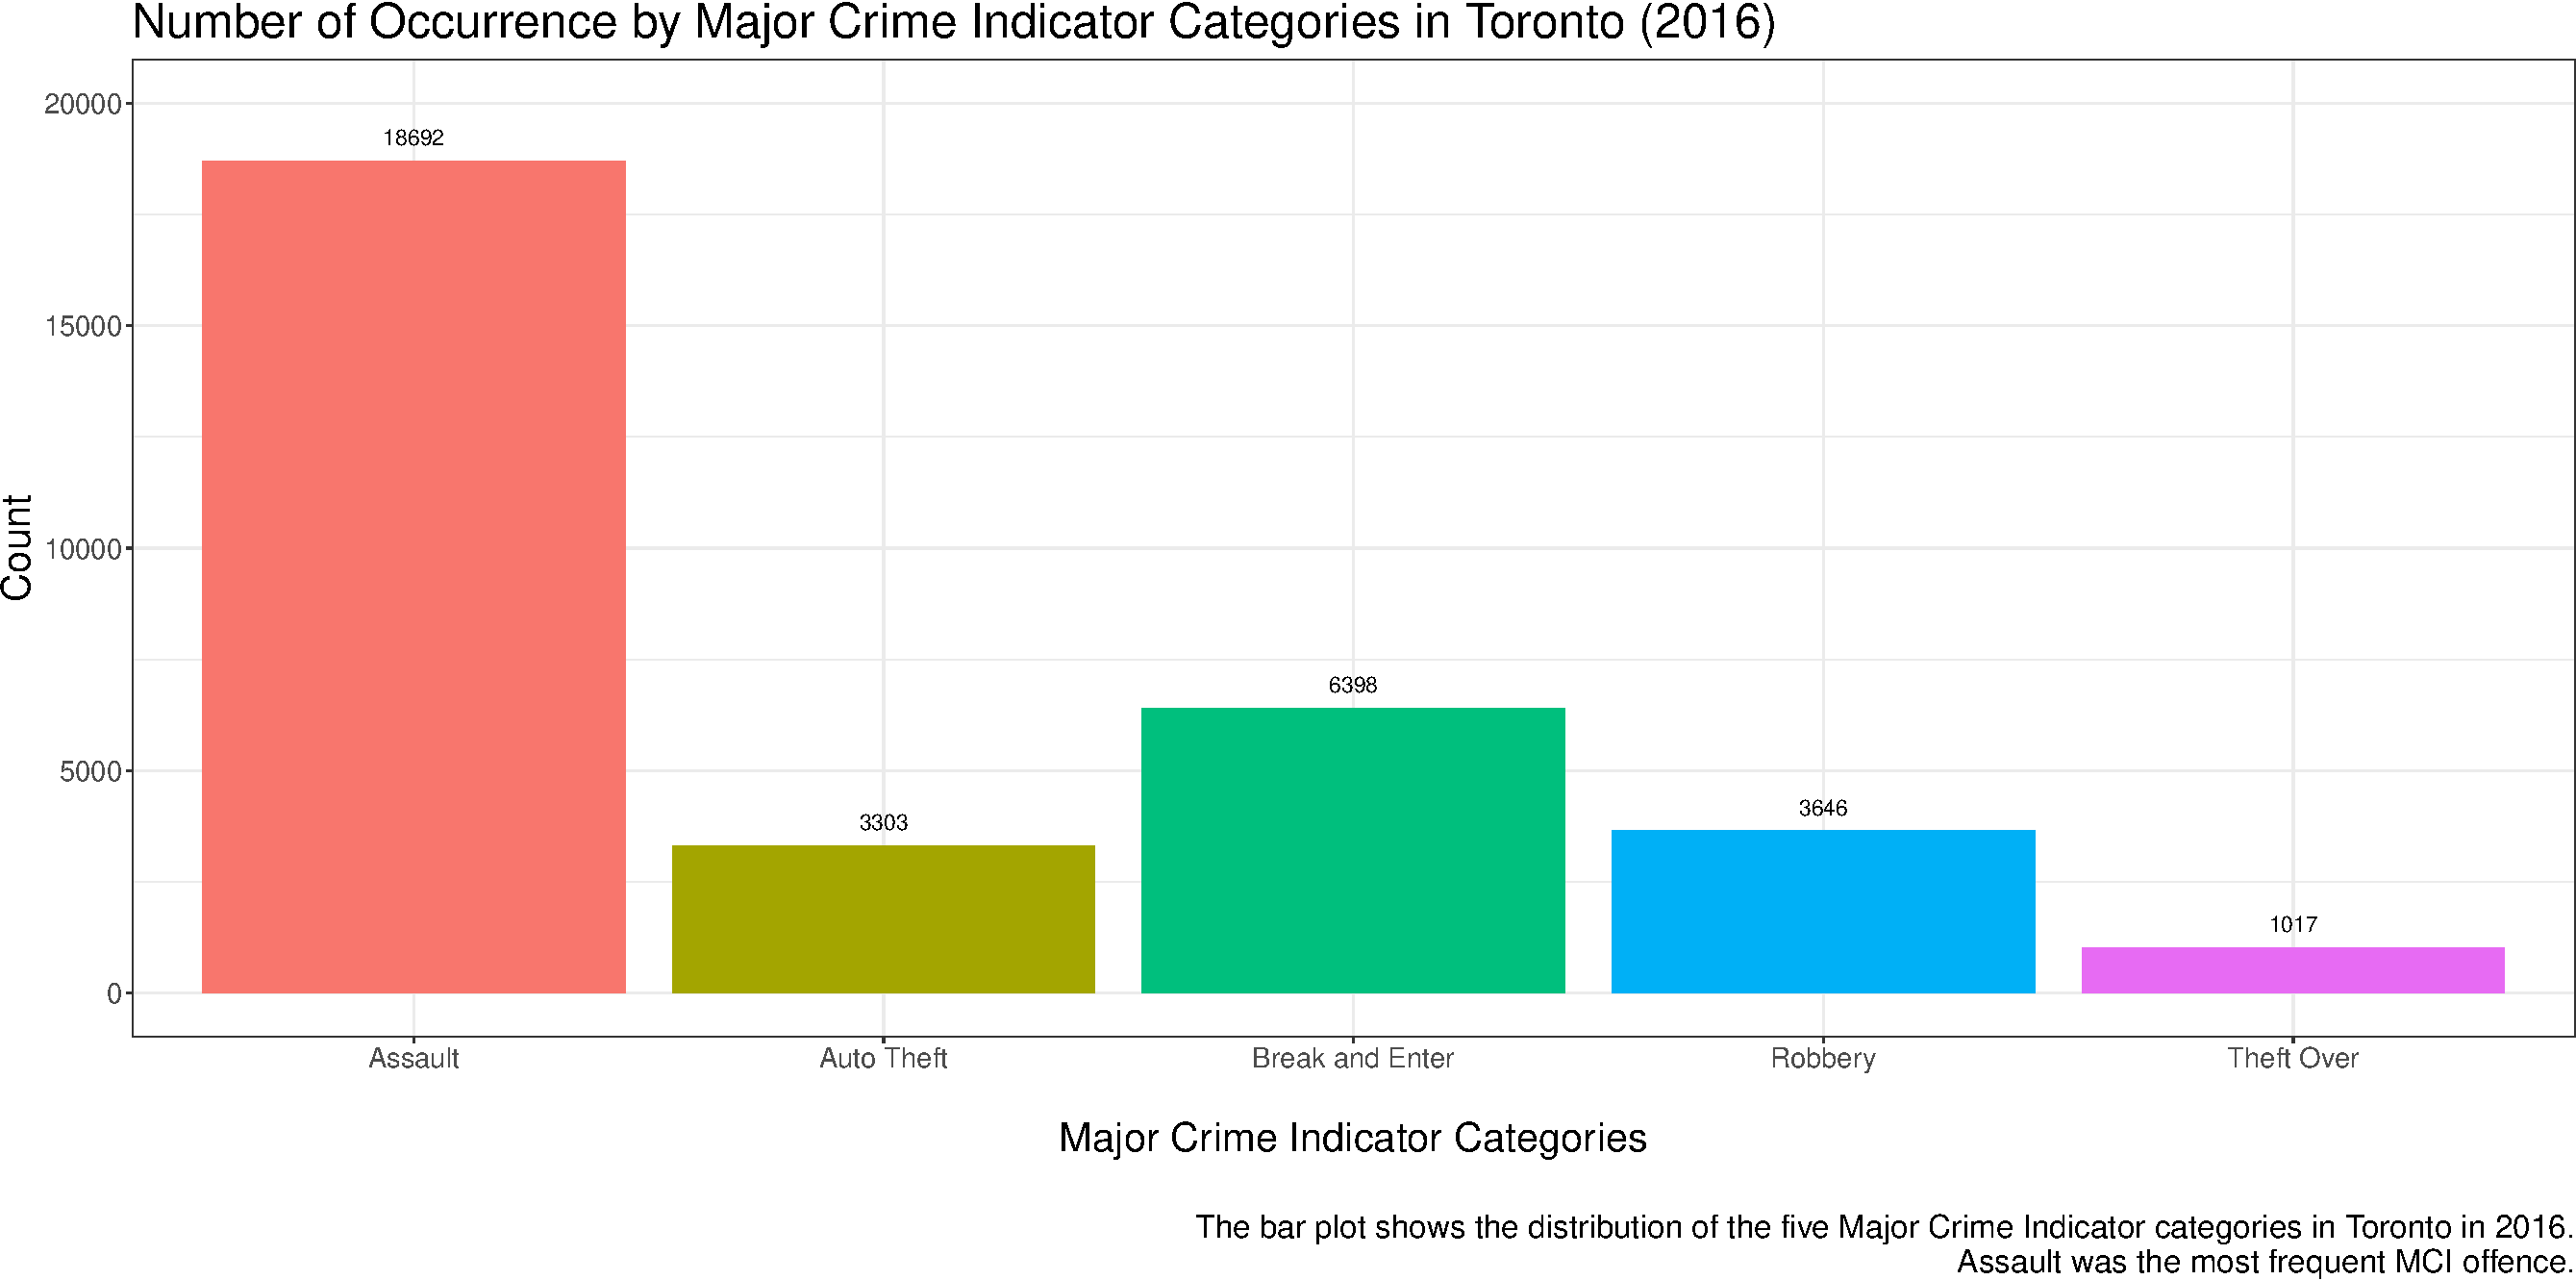
\includegraphics{Final-Report_files/figure-latex/crime-count-1.pdf}

The following stacked bar plots show the distribution of crime
occurrences and where they occurred. From these plots, there were some
interesting observations:

\begin{itemize}
\item
  ``Assault'' was the predominant crime in the seven premises type shown
  below, especially in Transit where it was about seven times more
  likely to occur than all the other four crimes. This suggested that
  neighbourhoods with large transit hubs were more likely to suffer from
  assault offences, or neighbourhoods with a higher population density
  (hence the need of more transit);
\item
  Neglecting ``Outside'', Commercial areas and Apartment buildings have
  the most MCI offences occurred. This might mean that areas such as
  downtown area with a high density of commercial properties and
  apartment buildings have a higher crime count than in relatively
  suburb areas with more houses.
\item
  Nearly half of the ``auto theft'' offences occurred outside. This
  suggested that neighbourhoods with more indoor or underground parking
  spaces might be less susceptible to auto theft
\item
  The number of crimes occurred in houses were about 80\% of that in
  apartments, but assuming that apartments usually house many more
  people than a house could, this suggested that the number of offences
  per person might be higher in houses (which appear in less busy areas)
  than apartments (which are often in city centers).
\end{itemize}

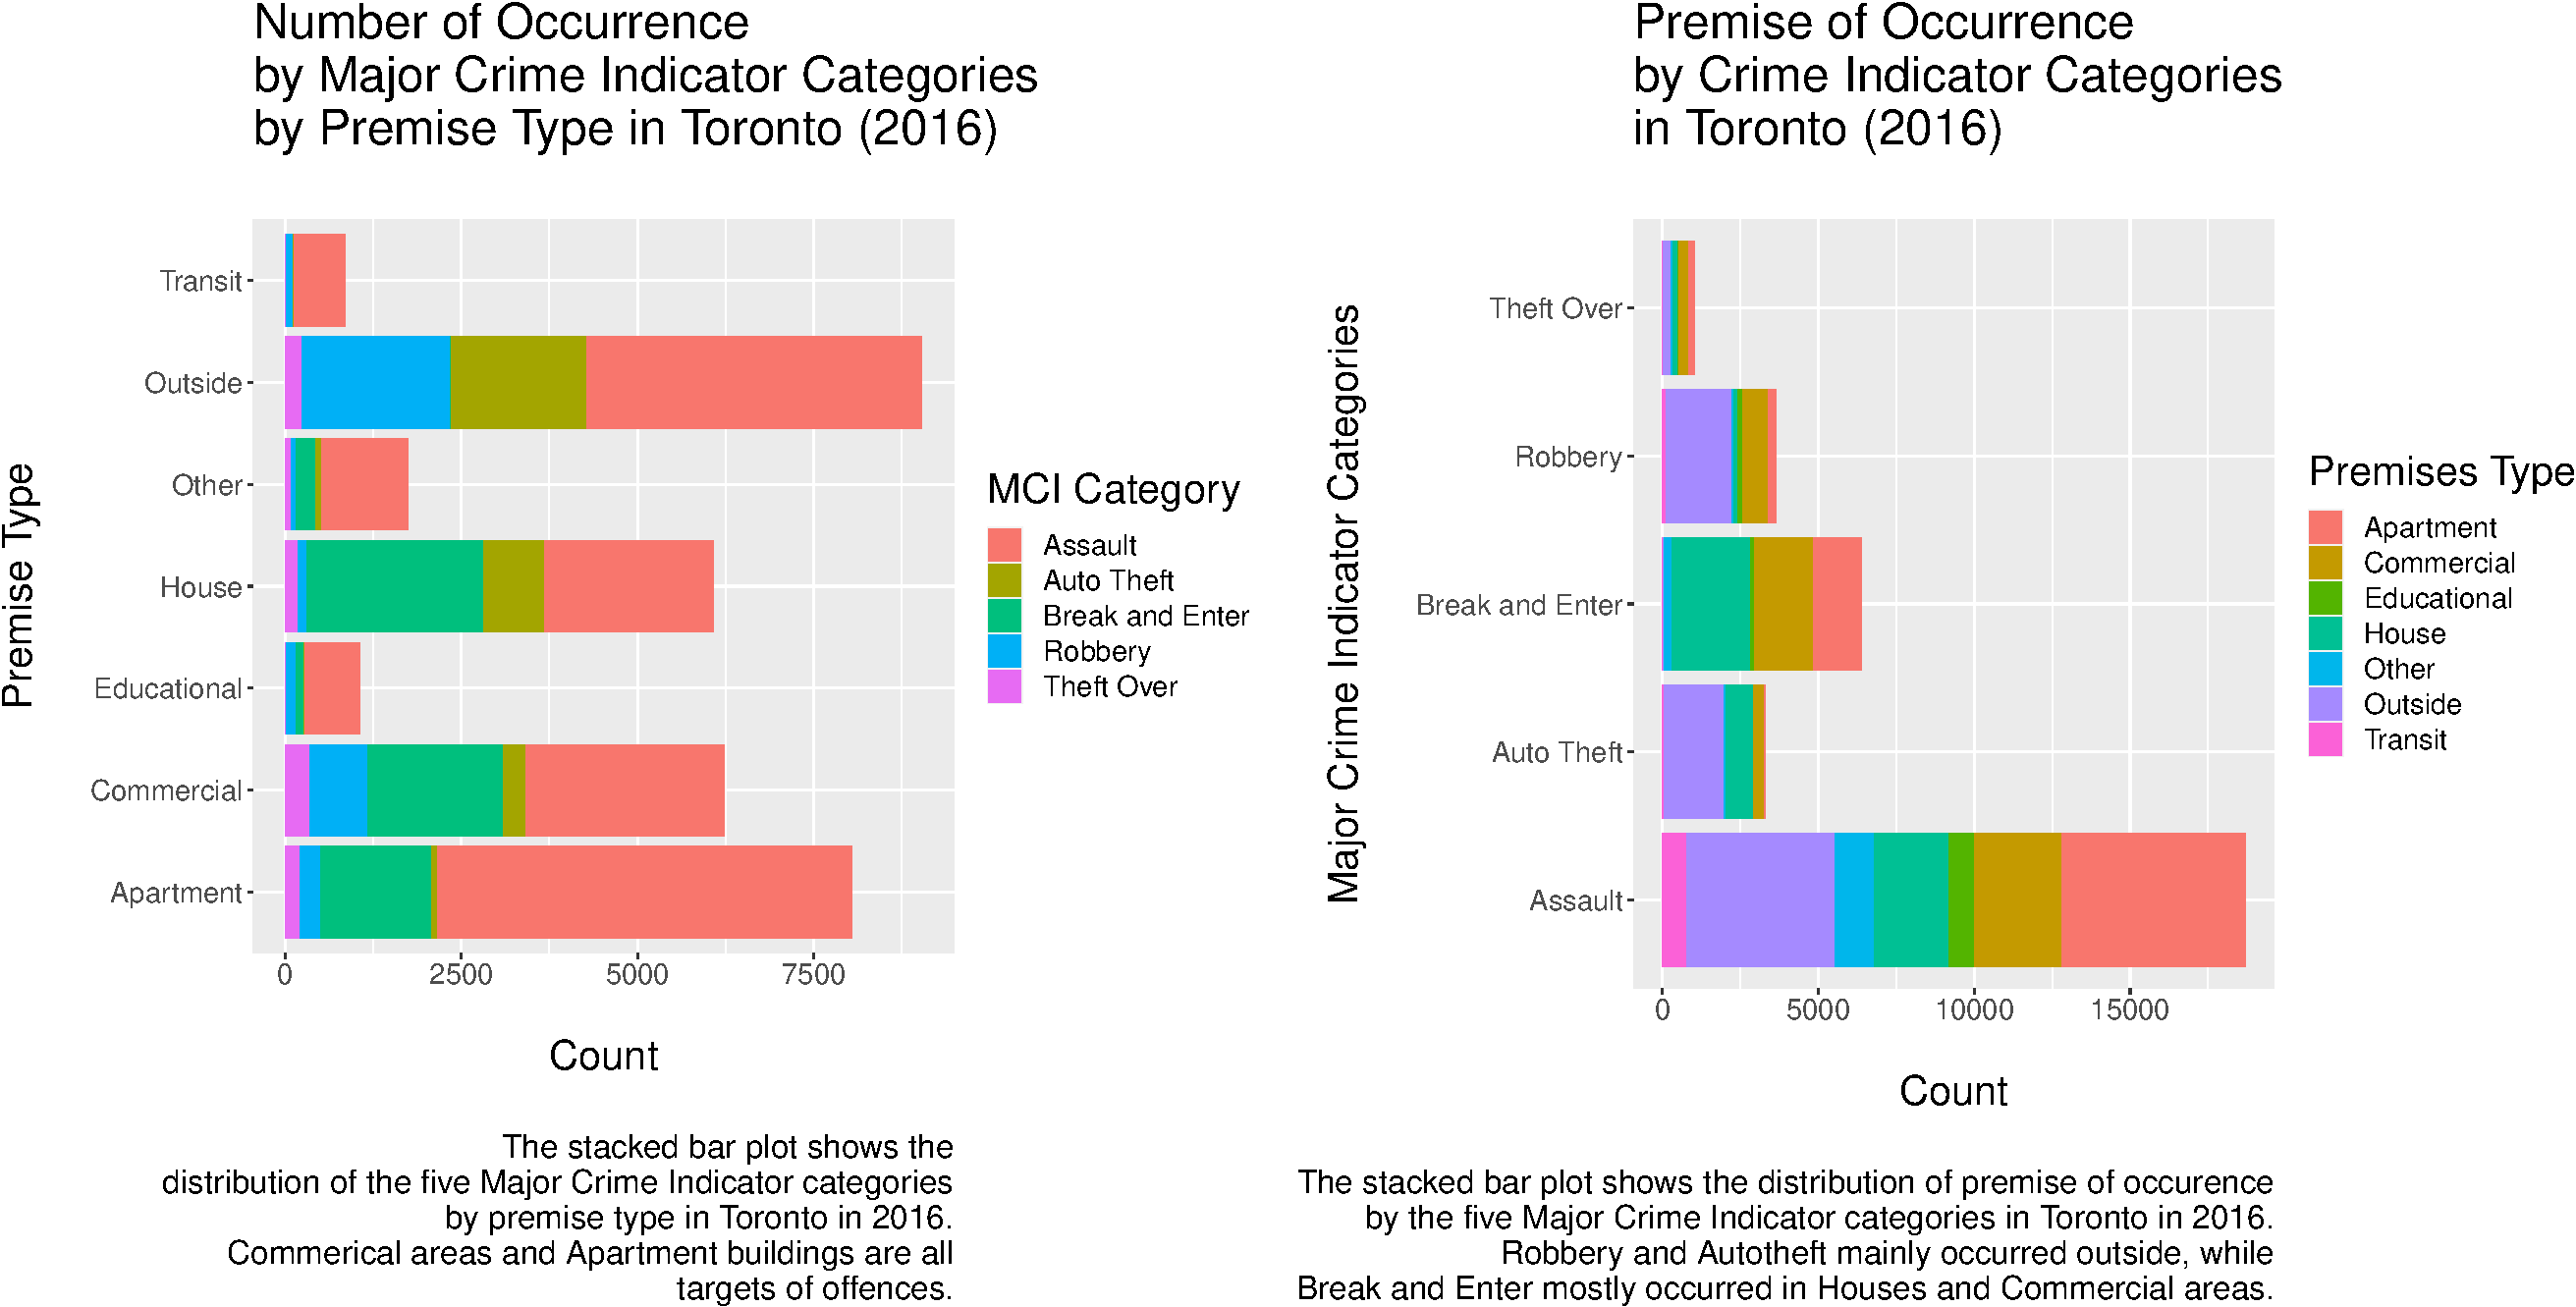
\includegraphics{Final-Report_files/figure-latex/crime-count-by-premise-1.pdf}

We also inspected the trend of offence occurrences with respect to time
in 2016 with the histogram below. The trend shown in the plot suggests
that there were no significant relationship between the day of year and
the number of major crime occurred, as the plot appears to be close to a
uniform distribution with only minor fluctuations periodically, with the
exception of Day 1: the spike of assault cases on the first day of the
year was interesting yet concerning. This spike does not seem to be from
a data collection error, as the dataset had valid information on all the
those cases on that day. This number might be related to new years
celebration where people usually got drunk and high during celebration
events and festivals, hence the increase in assault offences.

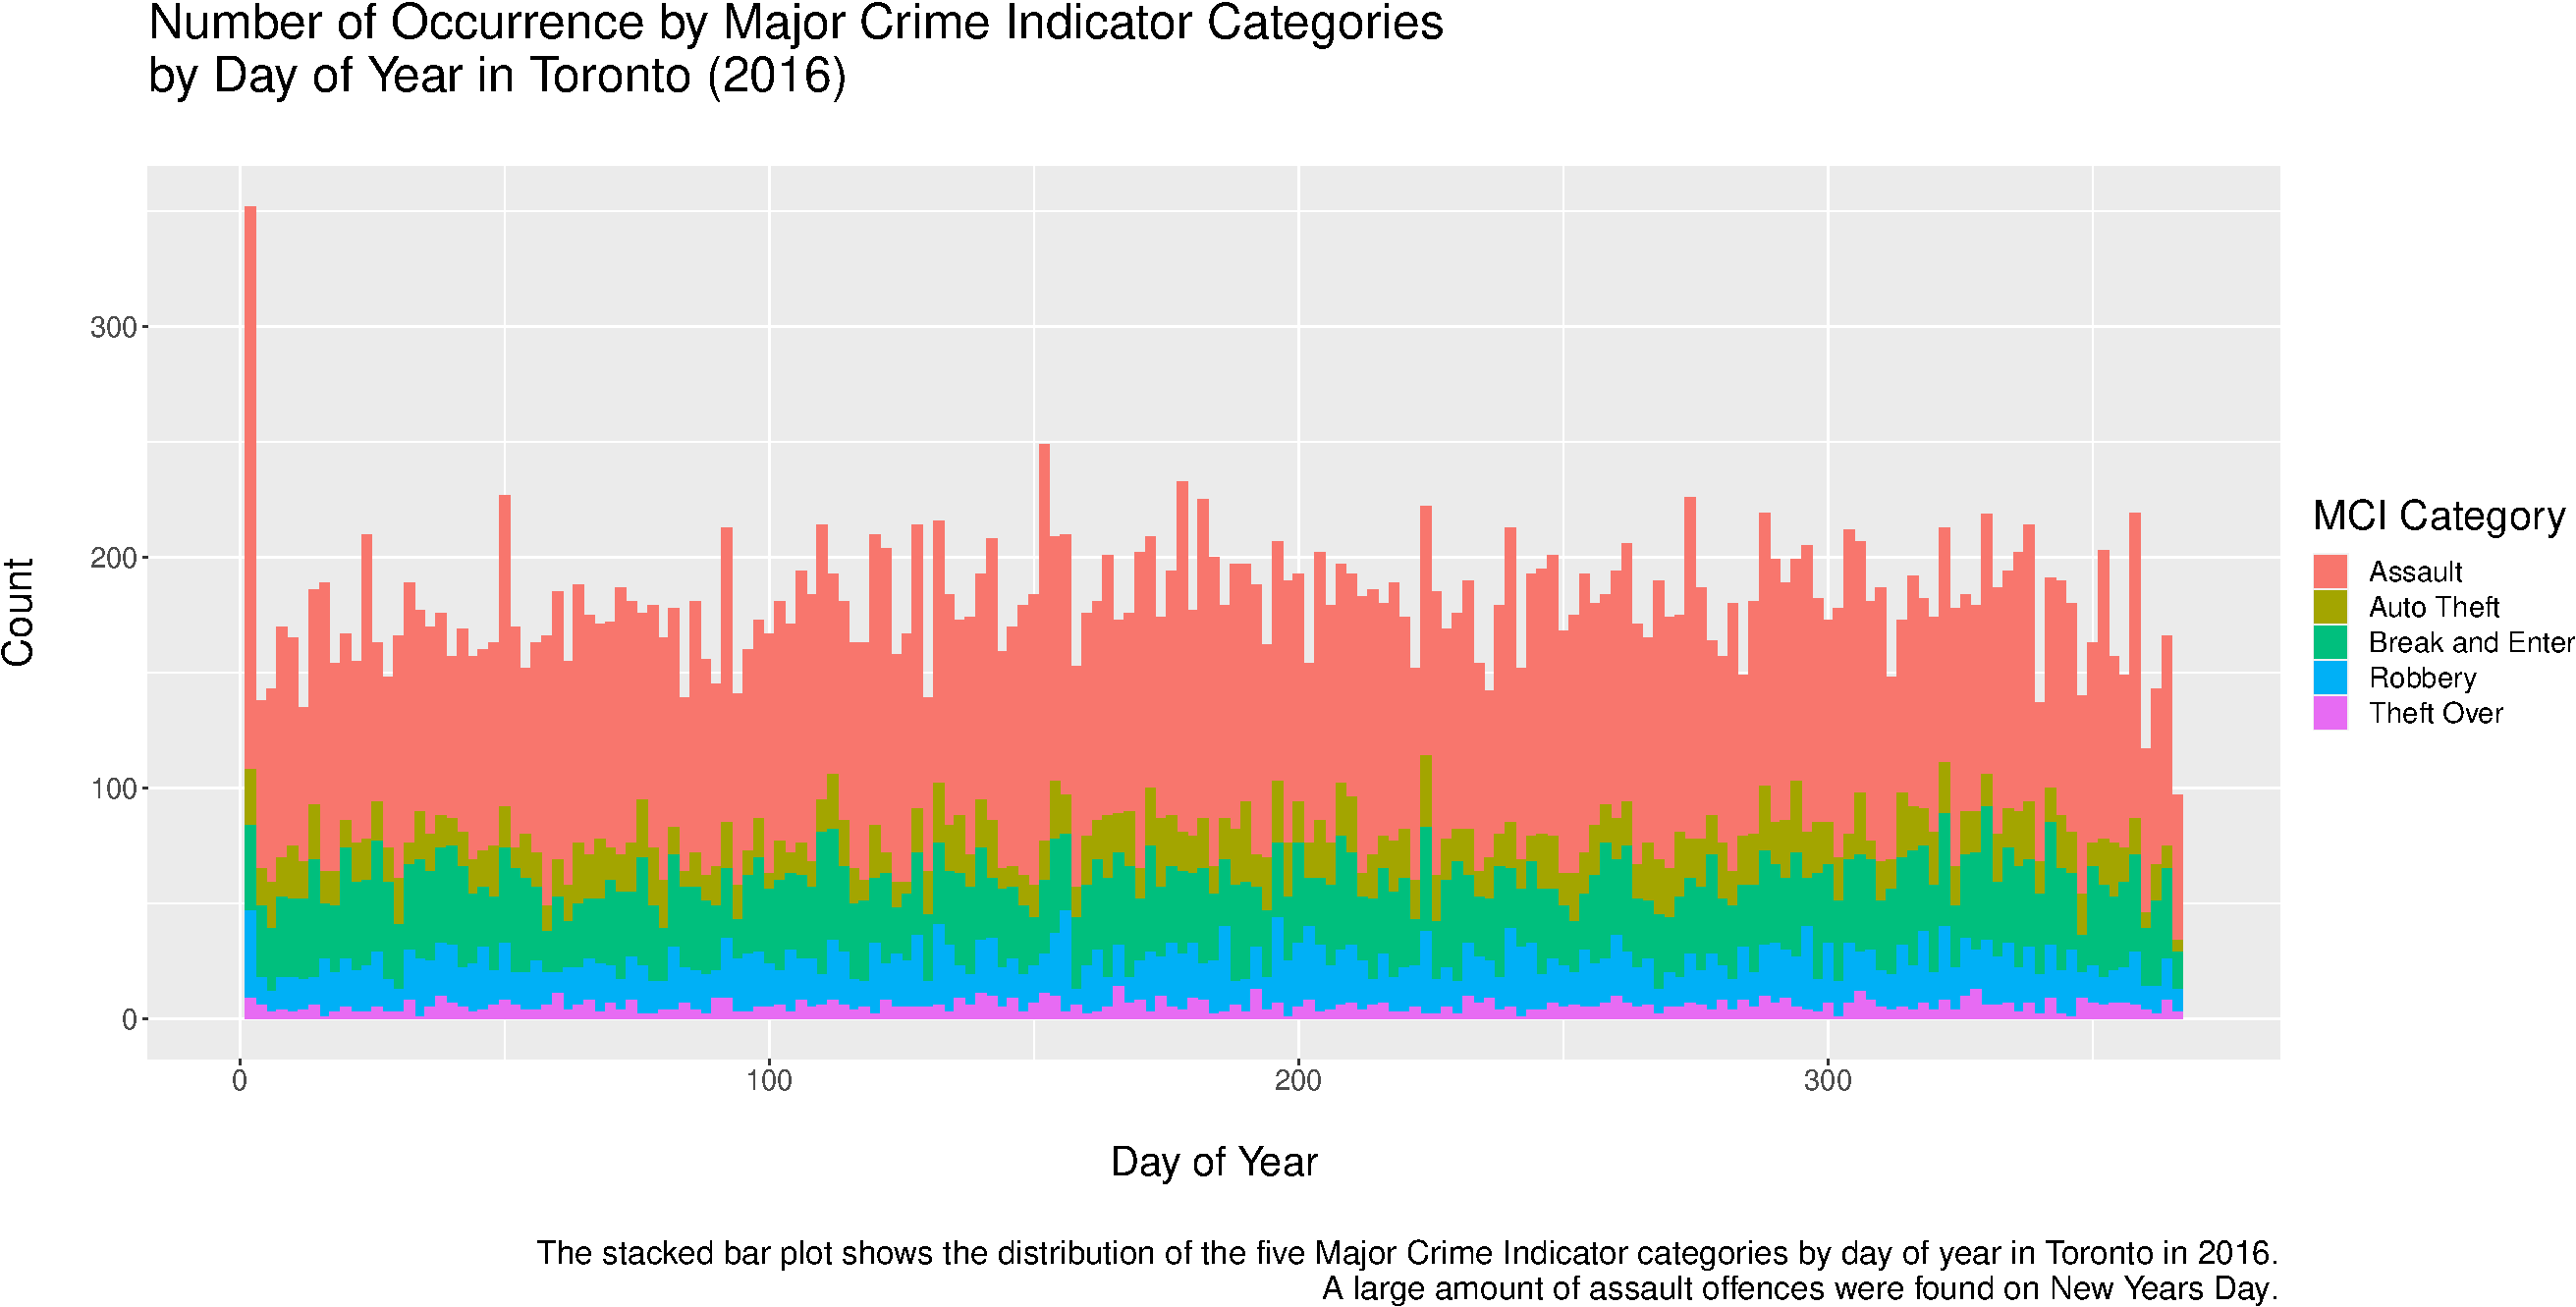
\includegraphics{Final-Report_files/figure-latex/crime-by-time-1.pdf}

The following barplot shows the Top 10 Neighbourhoods sorted by the
number of major crime occurrences in 2016 in descending order. The
results did not come as surprising, as the neighbourhood with the most
population (Waterfront Communities Population: 65913) had the highest
crime occurrences. Busy city centres were also in the plot (Bay Street,
Church-Yonge). Interestingly, West Humber Clairville had significantly
more auto theft offences compared to the other neighbourhoods, which was
80\% of all the other 9 neighbourhoods combined (318 vs 385).

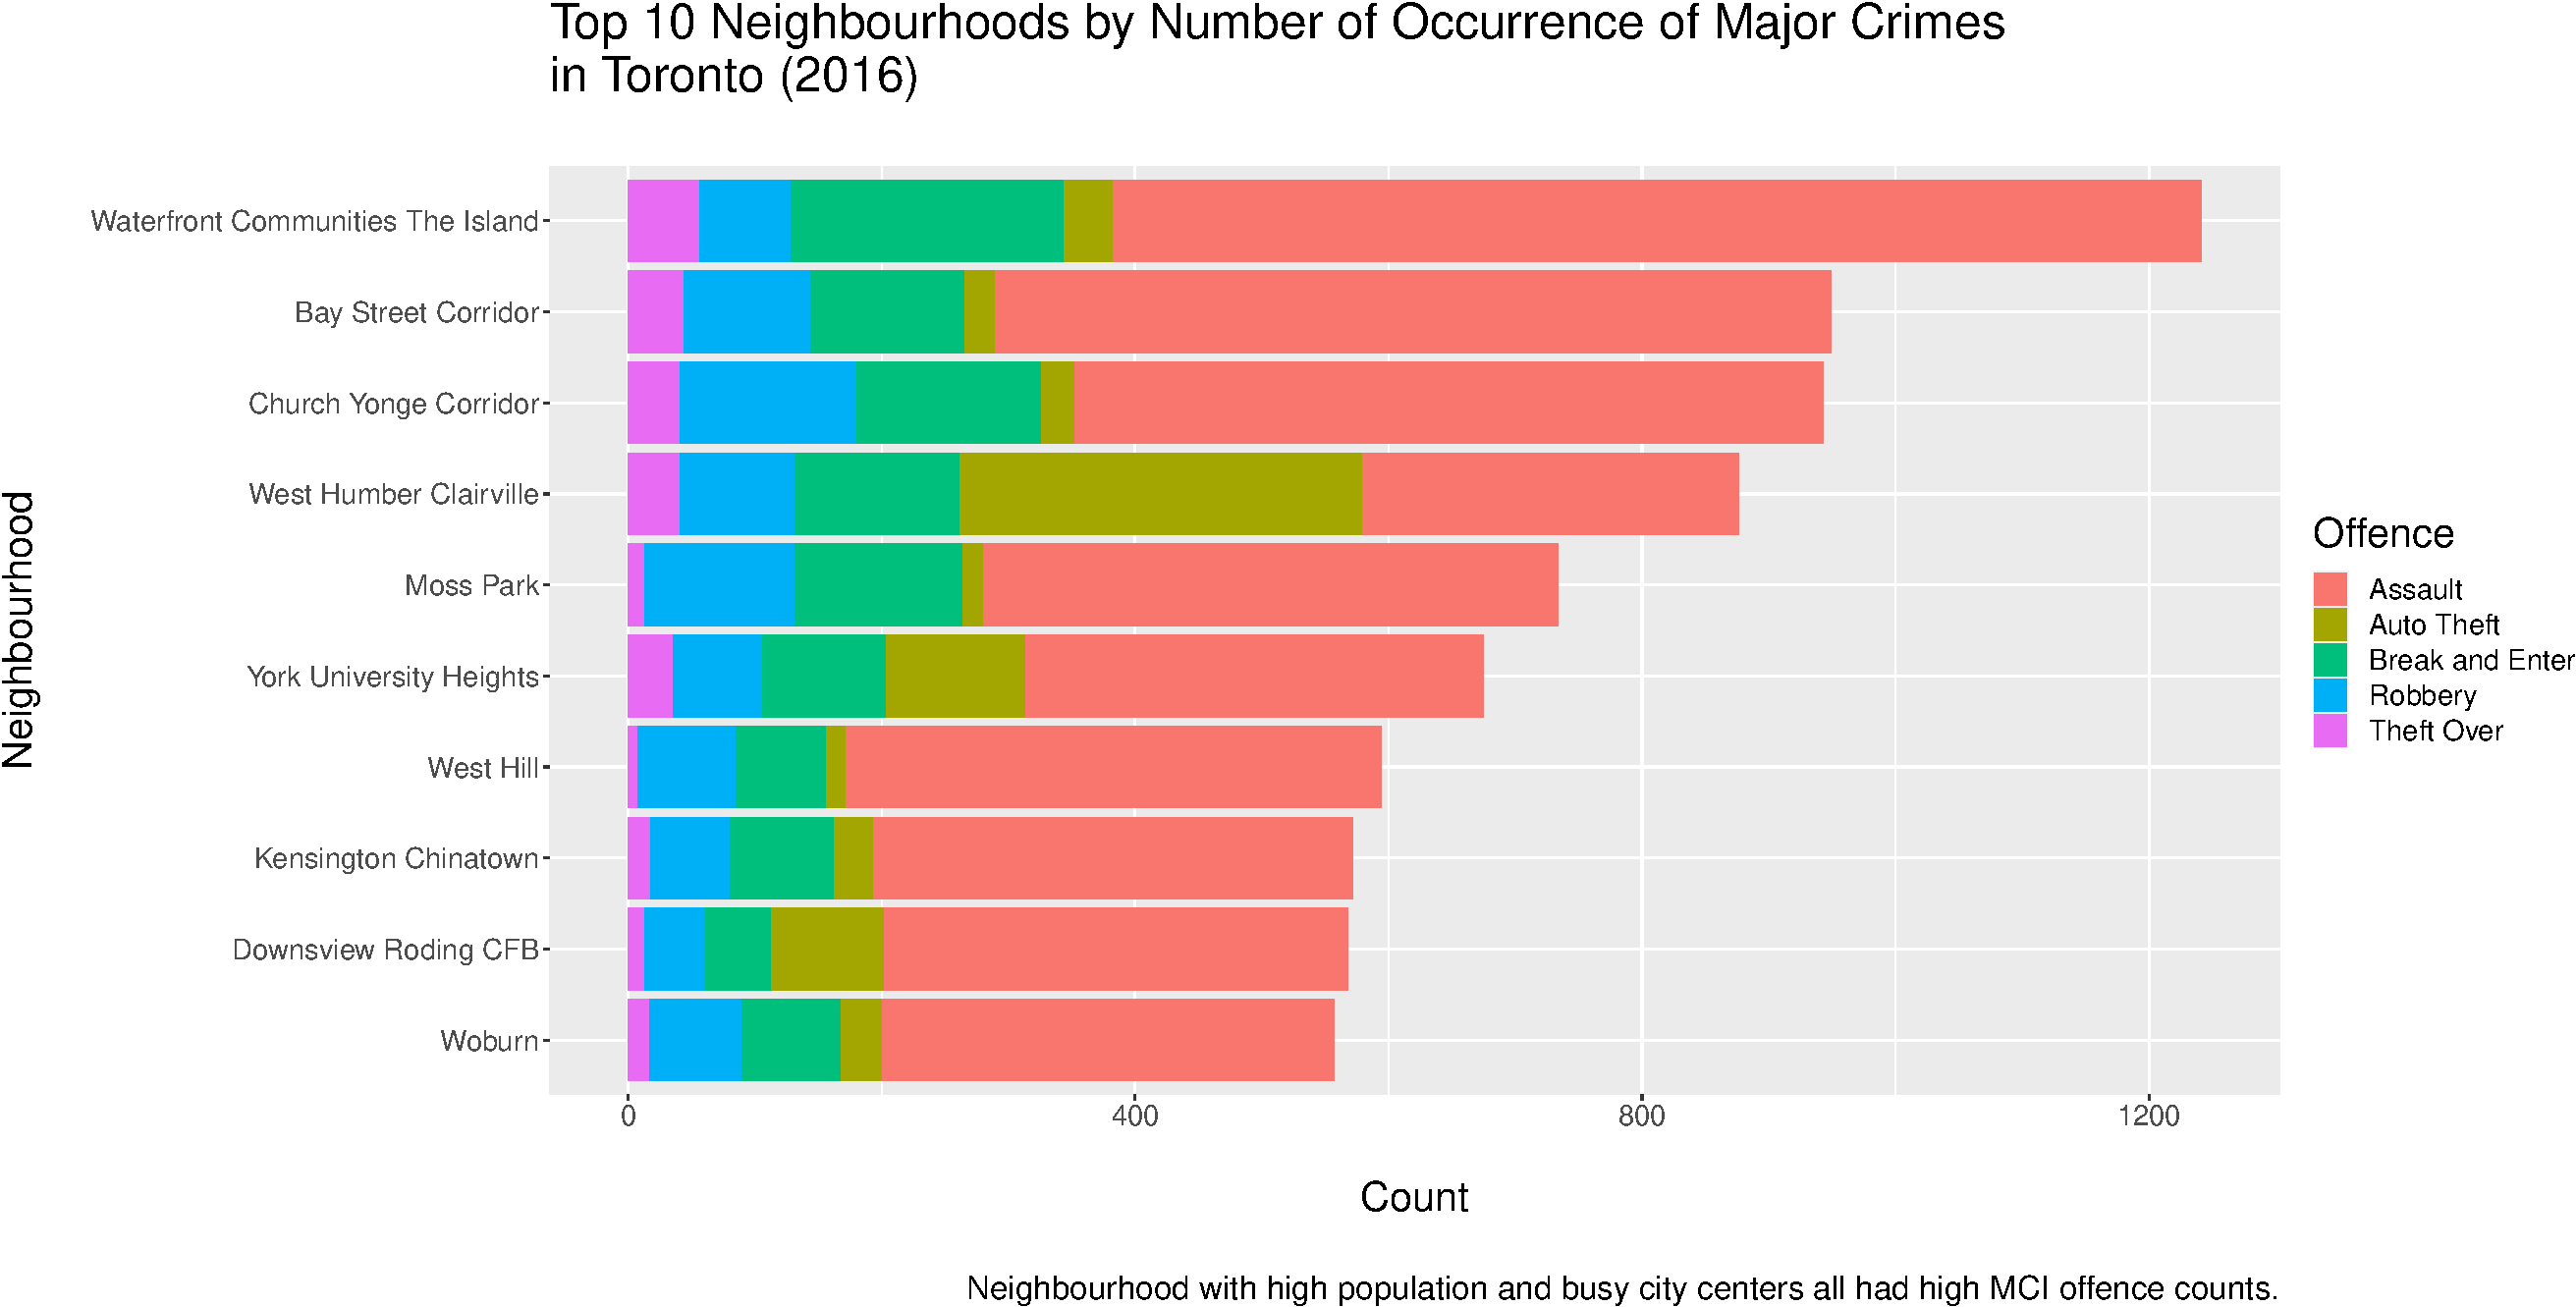
\includegraphics{Final-Report_files/figure-latex/crime-by-neighbourhood-1.pdf}

For more exploration on how the MCI offences were distributed in
Toronto's neighbourhoods, see the
\href{https://tyler-cy.github.io/JSC370-Final/Interactive-Visuals.html}{Interactive
Plots}.

\hypertarget{airbnb-listings-and-mci-offences}{%
\subsubsection{2.3.2 Airbnb Listings and MCI
Offences}\label{airbnb-listings-and-mci-offences}}

To investigate whether there was a correlation between the number of
Airbnb listings and MCI offences, a scatterplot with a best-fitted line
was created. The plot suggests that there is a moderate positive
relationship between these two numbers. However, the variance of number
of offences is much higher when the number of listings are high, which
suggests that Airbnb listing was only one of the factors which affected
the number of MCI offences.

Note that Waterfront Communities-The Island with 2754 listings and 1241
offences was omitted in the plot for aesthetic purposes.

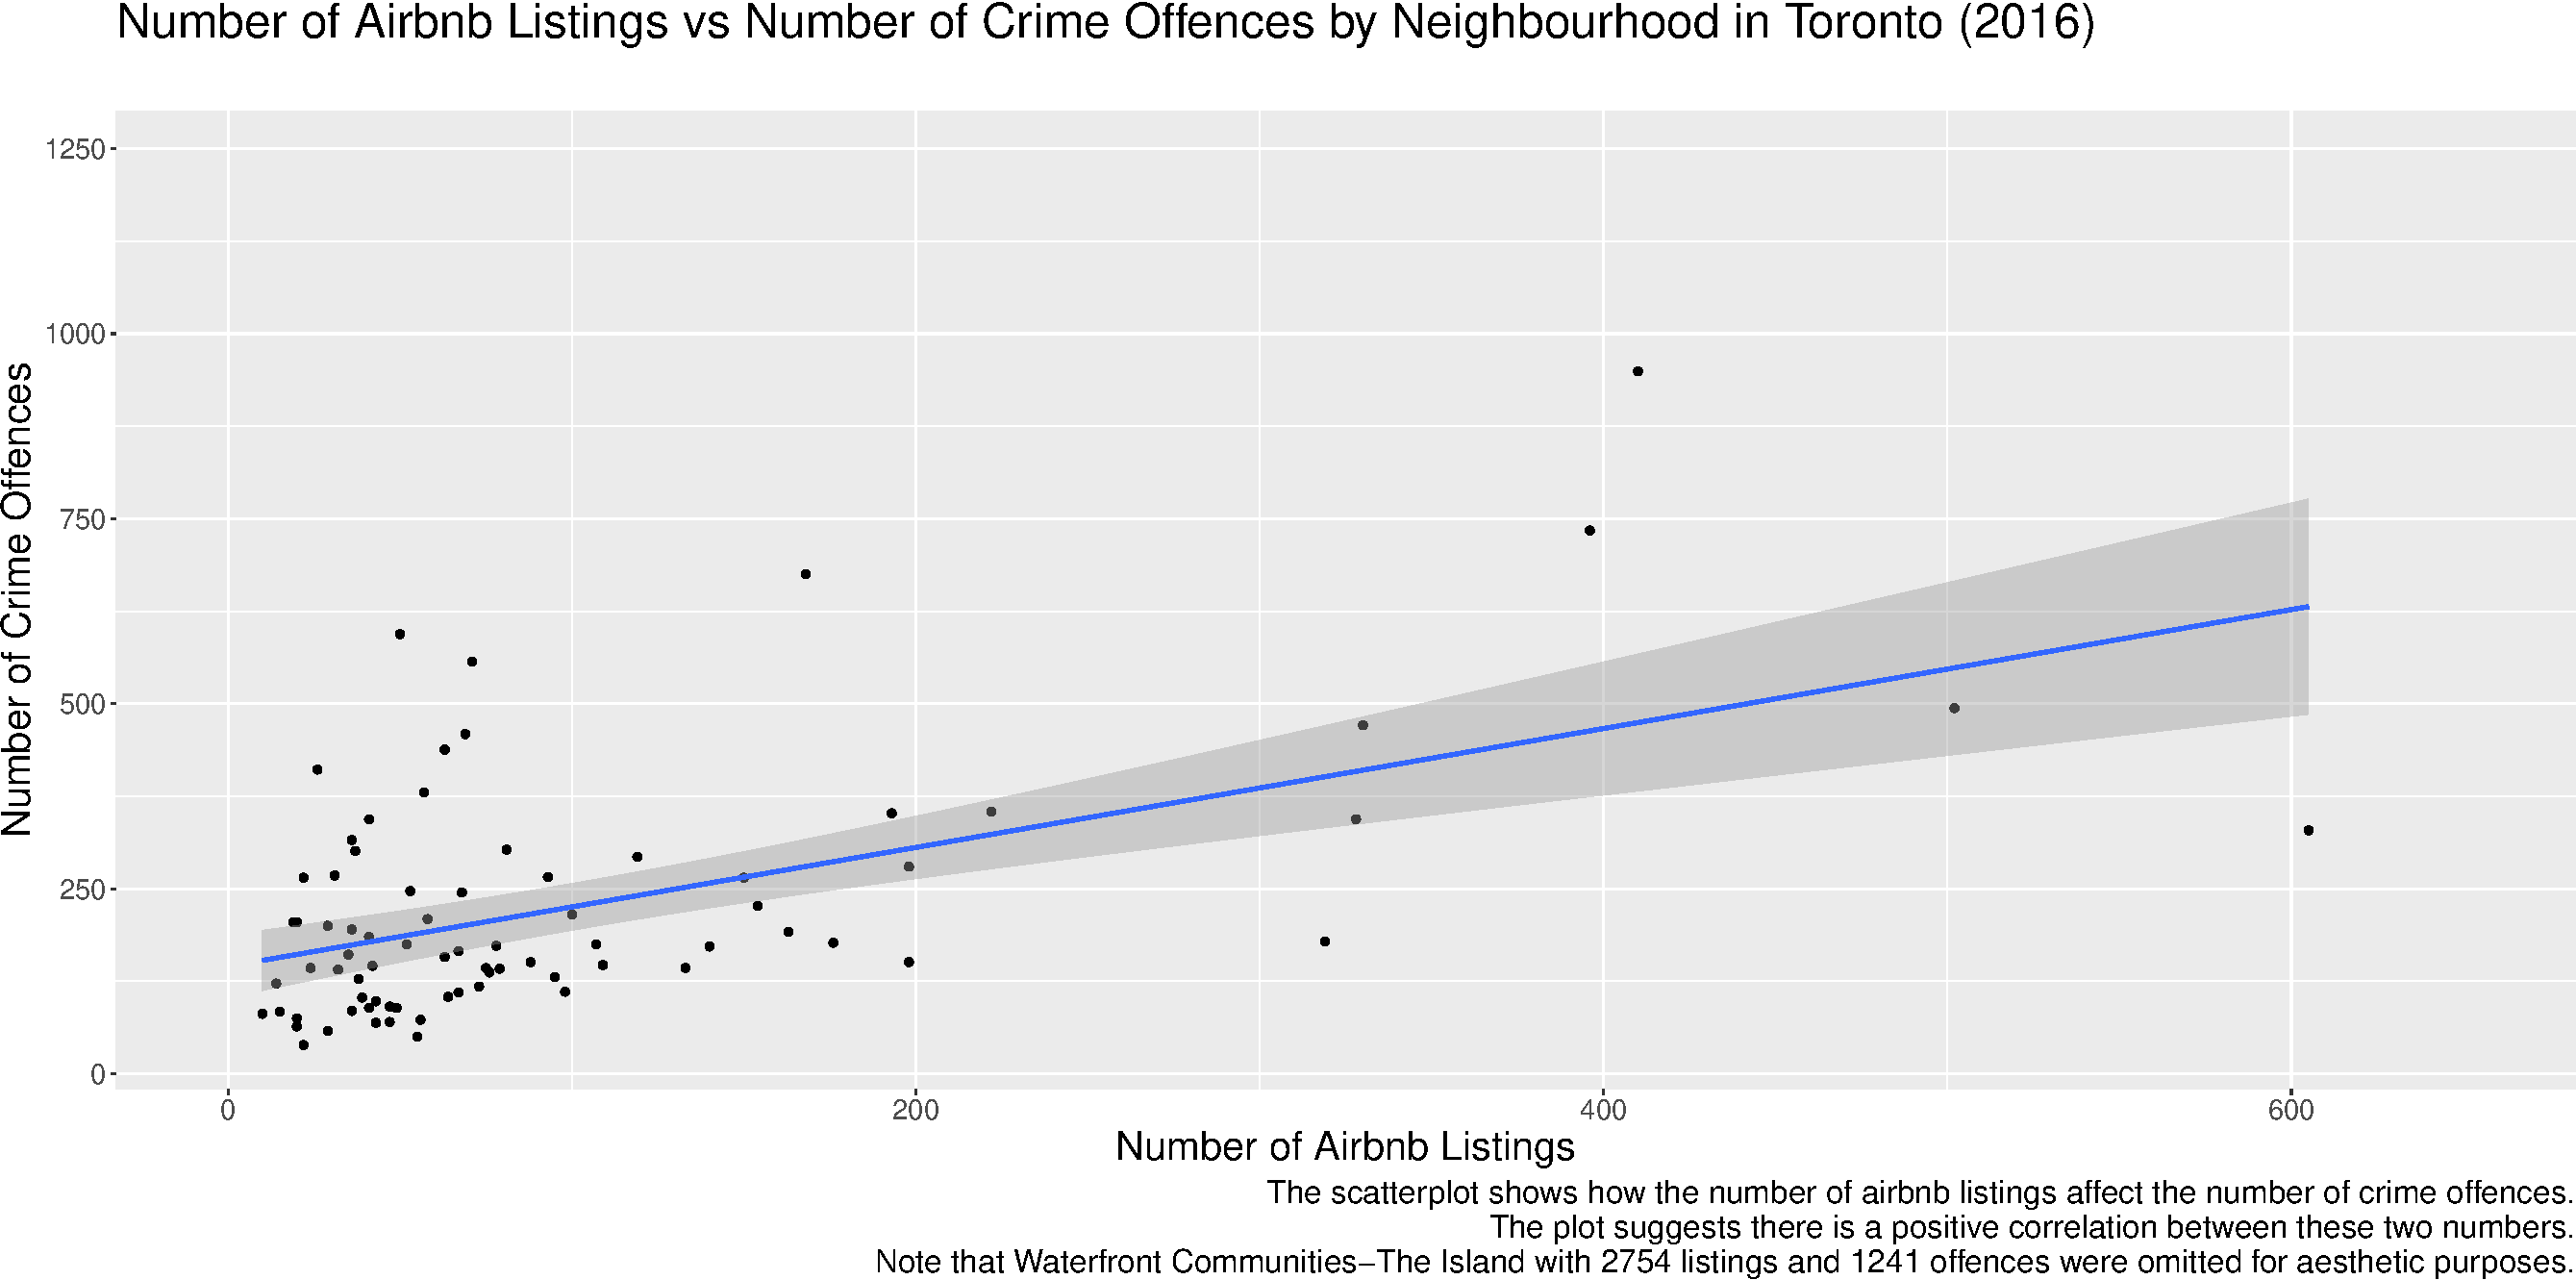
\includegraphics{Final-Report_files/figure-latex/airbnb_count-1.pdf}

\hypertarget{venues-pois-gyms-and-mci-offences}{%
\subsubsection{2.3.3 Venues (POIs), Gyms, and MCI
Offences}\label{venues-pois-gyms-and-mci-offences}}

Next, we investigated if the number of MCI offences were related to the
number of venues (POIs) and gyms by plotting a scatterplot with a
best-fitted line. There is only a very weak positive relationship
between these two factors, if not none at all. However, the plot shows
that some outliers with high number of MCI offences occurred in
neighbourhoods with the highest venues and gyms.

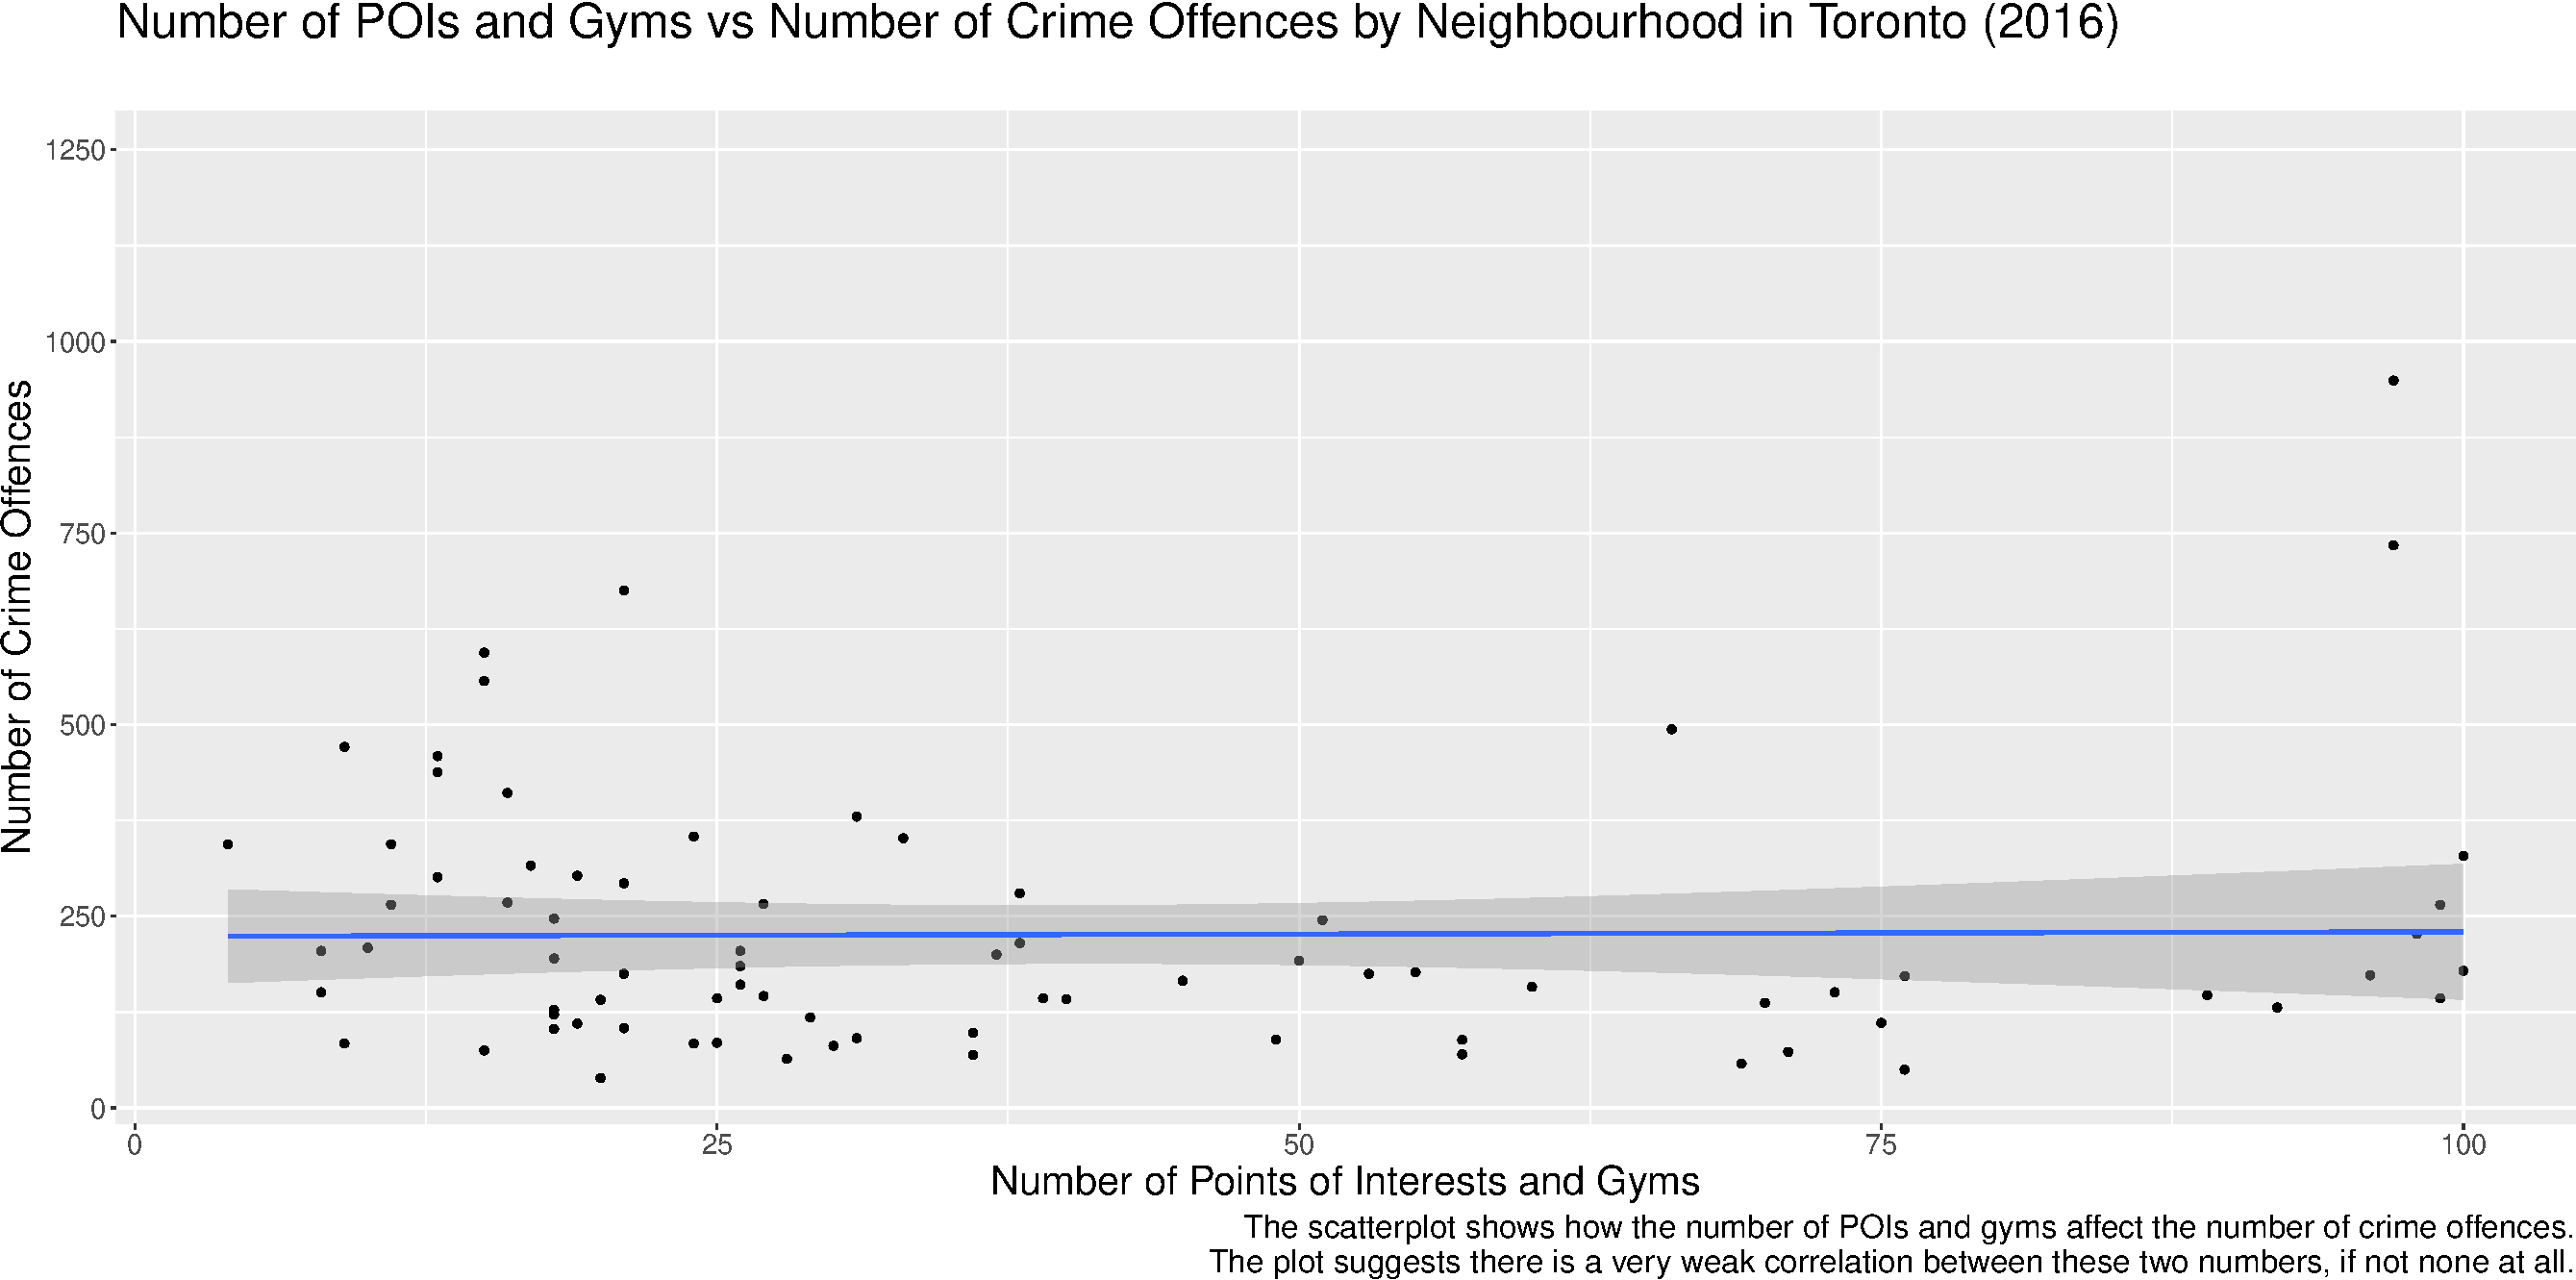
\includegraphics{Final-Report_files/figure-latex/venues_count-1.pdf}

\hypertarget{neighbourhood-demographics-and-crime-rate}{%
\subsubsection{2.3.4 Neighbourhood Demographics and Crime
Rate}\label{neighbourhood-demographics-and-crime-rate}}

We inspected the relationship between the crime rate and the variables
of interests, i.e.~population size, population age, education,
employment/labour, immigration and citizenship status, income taxes, and
the level of visible minority. For each variable, we used the extracted
sub-tables with only relevant fields created in the ``Data Cleaning''
section. For each sub-table, we merged it with two other tables, one
containing (Neighbourhood, Population) tuples, and one containing the
number of reported crime per offence type.

\hypertarget{relationship-between-population-size-and-crime-rate}{%
\paragraph{2.3.4.1 Relationship between Population Size and Crime
Rate}\label{relationship-between-population-size-and-crime-rate}}

It is not surprising that the best fitted lines shows that the number of
offences increased with the number of population in a neighbourhood.
However, in all the subplots, the majority of the neighbourhoods had a
population of less than 30 thousand, and there are outliers and
influential points in the plots. A better indicator of crime rate versus
population might be plotting the crime rate against the population
density instead, which is more representative of the scale of crime rate
in terms of neighbourhood size: a neighbourhood with higher population
density is more likely to have higher crime rate.

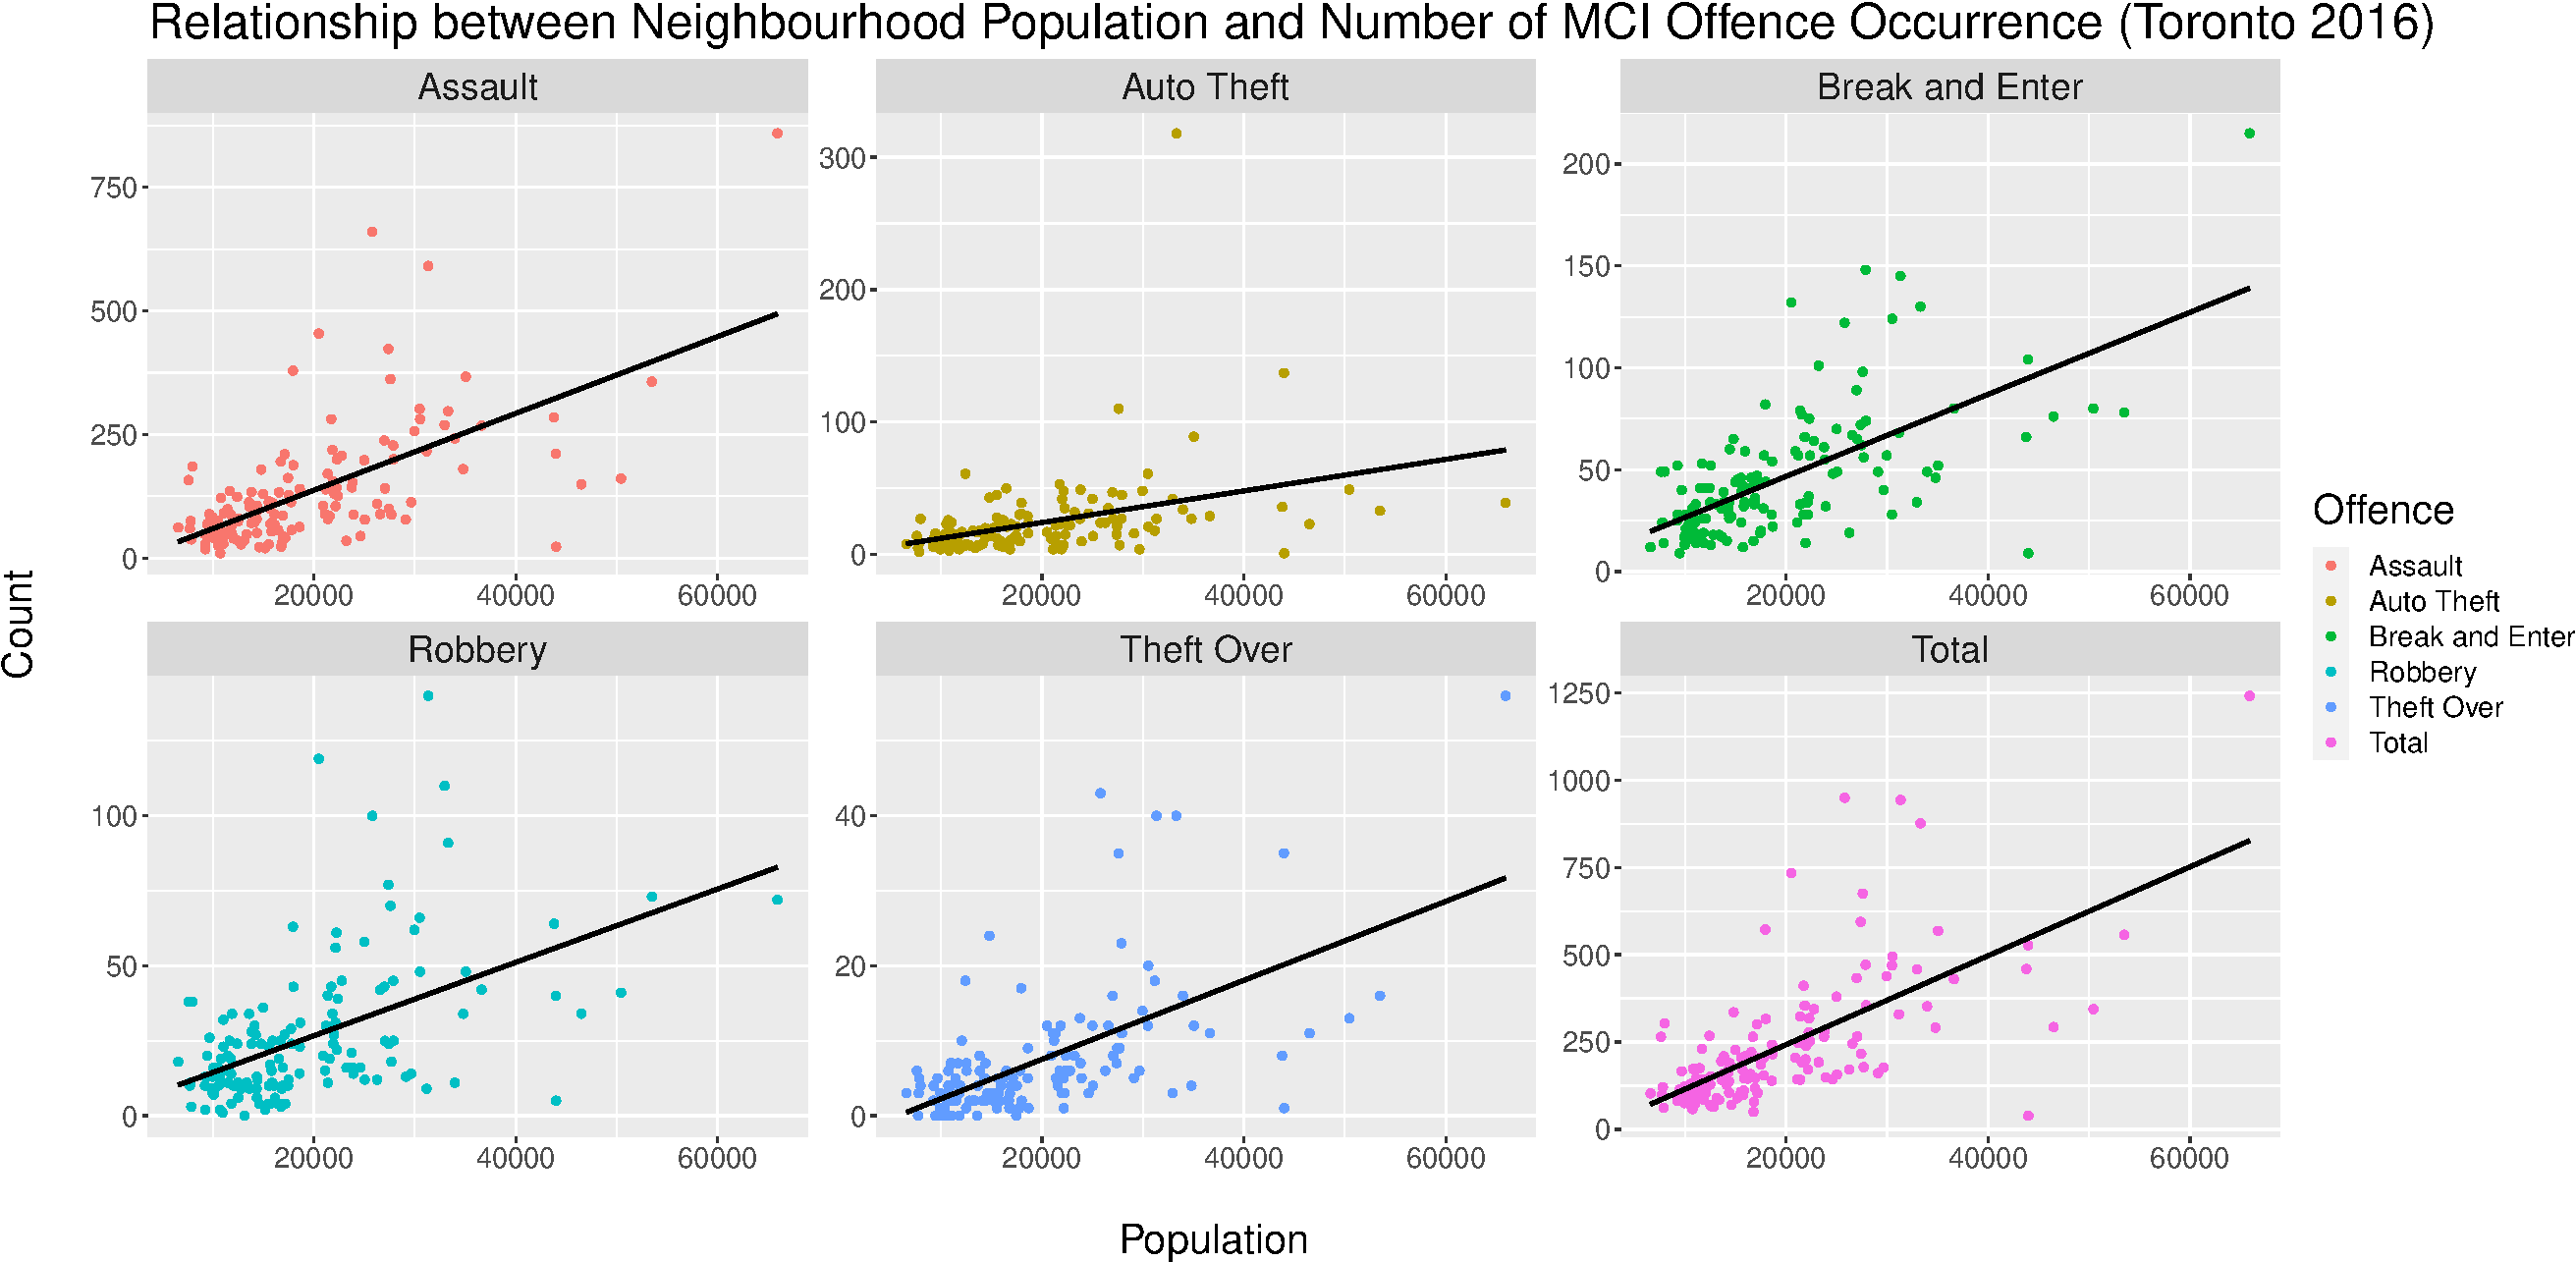
\includegraphics{Final-Report_files/figure-latex/crime-vs-population-2-1.pdf}

\hypertarget{relationship-between-population-age-and-crime-rate}{%
\paragraph{2.3.4.2 Relationship between Population Age and Crime
Rate}\label{relationship-between-population-age-and-crime-rate}}

We fitted a basic linear model where the response variable was the
number of offences and the variables were the proportion of different
age groups in the neighbourhood. Note that in the original dataset,
there were two additional age groups (Seniors (65+ years) and Older
Seniors (85+ years)). However, we did not include them in this
preliminary model as it would induce multicollinearity, since these
proportions of age groups add up to 1.

From the p-values below, we can see that the proportion of age groups
are all statistically significant. Based on the signs of the estimated
coefficients, they confirm from our previous findings that a
neighbourhood with larger proportion of senior residents are likely to
have fewer crime rate (negative coefficient), while increasing number of
youths (positive coefficient) is more likely to the crime
rate\footnote{Ulmer, J. T., \& Steffensmeier, D. (2014). The age and
  crime relationship: Social variation, social explanations. In The
  Nurture Versus Biosocial Debate in Criminology: On the Origins of
  Criminal Behavior and Criminality (pp.~377-396). SAGE Publications
  Inc.. \url{https://doi.org/10.4135/9781483349114.n23}}.

However, the estimated coefficient for the intercept is much larger than
the estimated coefficient for the age groups, thus any change in the
percentages of age groups would only change the estimated crime rate
slightly. This strongly suggested that there were other factors which
affect crime rate, and the p-values show that age group is one of the
significant factors.

\begin{table}

\caption{\label{tab:crime-vs-age-lm}Coefficient Estimates of a Linear Regression Model for Estimating MCI Offence Count (Age Groups)}
\centering
\begin{tabular}[t]{l|r|r|r|r}
\hline
Terms & Estimate & Std. Error & t-value & p-value\\
\hline
(Intercept) & 57.993 & 21.730 & 2.669 & 0.009\\
\hline
`Children (0-14 years)` & -0.032 & 0.012 & -2.660 & 0.009\\
\hline
`Youth (15-24 years)` & 0.125 & 0.015 & 8.320 & 0.000\\
\hline
`Working Age (25-54 years)` & 0.014 & 0.003 & 4.286 & 0.000\\
\hline
`Pre-retirement (55-64 years)` & -0.065 & 0.019 & -3.351 & 0.001\\
\hline
\end{tabular}
\end{table}

\hypertarget{relationship-between-education-and-crime-rate}{%
\paragraph{2.3.4.3 Relationship between Education and Crime
Rate}\label{relationship-between-education-and-crime-rate}}

We also fitted a basic linear model where the response variable is the
number of MCI offences and the predictors are the proprtion of people
with different levels of education. The baseline of education is ``No
certificate, diploma or degree''. From the summary, we can see that an
increase proportion of people with secondary and postsecondary education
increases the number of crime rates, but the increase is around 3 times
as big for an increase in proportion of people with only secondary
education than those with postsecondary education.

Similar to the estimated coefficients for age groups, the estimated
coefficient for the intercept (-581) is negative and the estimated
coefficients for the factors were positive and much larger (708 and
2299). This strongly suggested that we should also look at other factors
at the same time. The p-values suggest that education is a significant
factor on crime rate alone, so it might be useful to combine education
with other variables and check if the combinations affect crime rate
altogether.

\begin{table}

\caption{\label{tab:crime-vs-education-lm}Coefficient Estimates of a Linear Regression Model for Estimating MCI Offence Count (Education)}
\centering
\begin{tabular}[t]{l|r|r|r|r}
\hline
Terms & Estimate & Std. Error & t-value & p-value\\
\hline
(Intercept) & -581.034 & 256.482 & -2.265 & 0.025\\
\hline
`  Postsecondary certificate, diploma or degree` & 708.739 & 250.138 & 2.833 & 0.005\\
\hline
`  Secondary (high) school diploma or equivalency certificate` & 2299.184 & 711.735 & 3.230 & 0.002\\
\hline
\end{tabular}
\end{table}

\hypertarget{relationship-between-employment-and-crime-rate}{%
\paragraph{2.3.4.4 Relationship between Employment and Crime
Rate}\label{relationship-between-employment-and-crime-rate}}

The fitted linear model below shows that the effect of the number of
people who did not work in a neighbourhood on crime rate was
statistically significant. This result aligned with the common consensus
that unemployment rate was positively correlated with crime rate
(Farrington et al.~1986\footnote{Farrington, D. P., Gallagher, B.,
  Morley, L., St.~Ledger, R. J., \& West, D. J. (1986). UNEMPLOYMENT,
  SCHOOL LEAVING, AND CRIME. The British Journal of Criminology, 26(4),
  335--356. \url{http://www.jstor.org/stable/23637076}}, John Howard
Society of Ontario 2009\footnote{\url{https://johnhoward.on.ca/wp-content/uploads/2014/09/facts-24-crime-and-unemployment-whats-the-link-march-2009.pdf}}).

\begin{table}

\caption{\label{tab:crime-vs-employment-lm}Coefficient Estimates of a Linear Regression Model for Estimating MCI Offence Count (Employment Status)}
\centering
\begin{tabular}[t]{l|r|r|r|r}
\hline
Terms & Estimate & Std. Error & t-value & p-value\\
\hline
(Intercept) & 57.258 & 28.187 & 2.031 & 0.044\\
\hline
`  Did not work` & 0.032 & 0.004 & 7.282 & 0.000\\
\hline
\end{tabular}
\end{table}

\hypertarget{relationship-between-immigration-and-citizenship-status-and-crime-rate}{%
\paragraph{2.3.4.5 Relationship between Immigration and Citizenship
Status and Crime
Rate}\label{relationship-between-immigration-and-citizenship-status-and-crime-rate}}

We plotted the number of MCI offences against the proprtion of
immigrants in the 140 neighbourhoods, separated by offence type and also
included a total count. From these plots, we can see that as the
proportion of immigrants increased in a neighbourhood, the number of
crimes committed decreases, with the exception of ``Break and Enter''
which stayed roughly the same. This aligned with our prior findings
which concluded that the number of immigrants
(statistically-)significantly reduced the number of crimes in the
area\footnote{Statistics Canada. (n.d.). Main article. Neighbourhood
  Characteristics and the Distribution of Police-reported Crime in the
  City of Toronto. Retrieved March 13, 2023, from
  \url{https://www150.statcan.gc.ca/n1/pub/85-561-m/2009018/part-partie1-eng.htm}}.

\begin{table}

\caption{\label{tab:crime-vs-immigration-lm}Coefficient Estimates of a Linear Regression Model for Estimating MCI Offence Count (Employment Status)}
\centering
\begin{tabular}[t]{l|r|r|r|r}
\hline
Terms & Estimate & Std. Error & t-value & p-value\\
\hline
(Intercept) & 378.555 & 59.861 & 6.324 & 0.000\\
\hline
Immigration\_Rate & -278.403 & 112.786 & -2.468 & 0.015\\
\hline
\end{tabular}
\end{table}

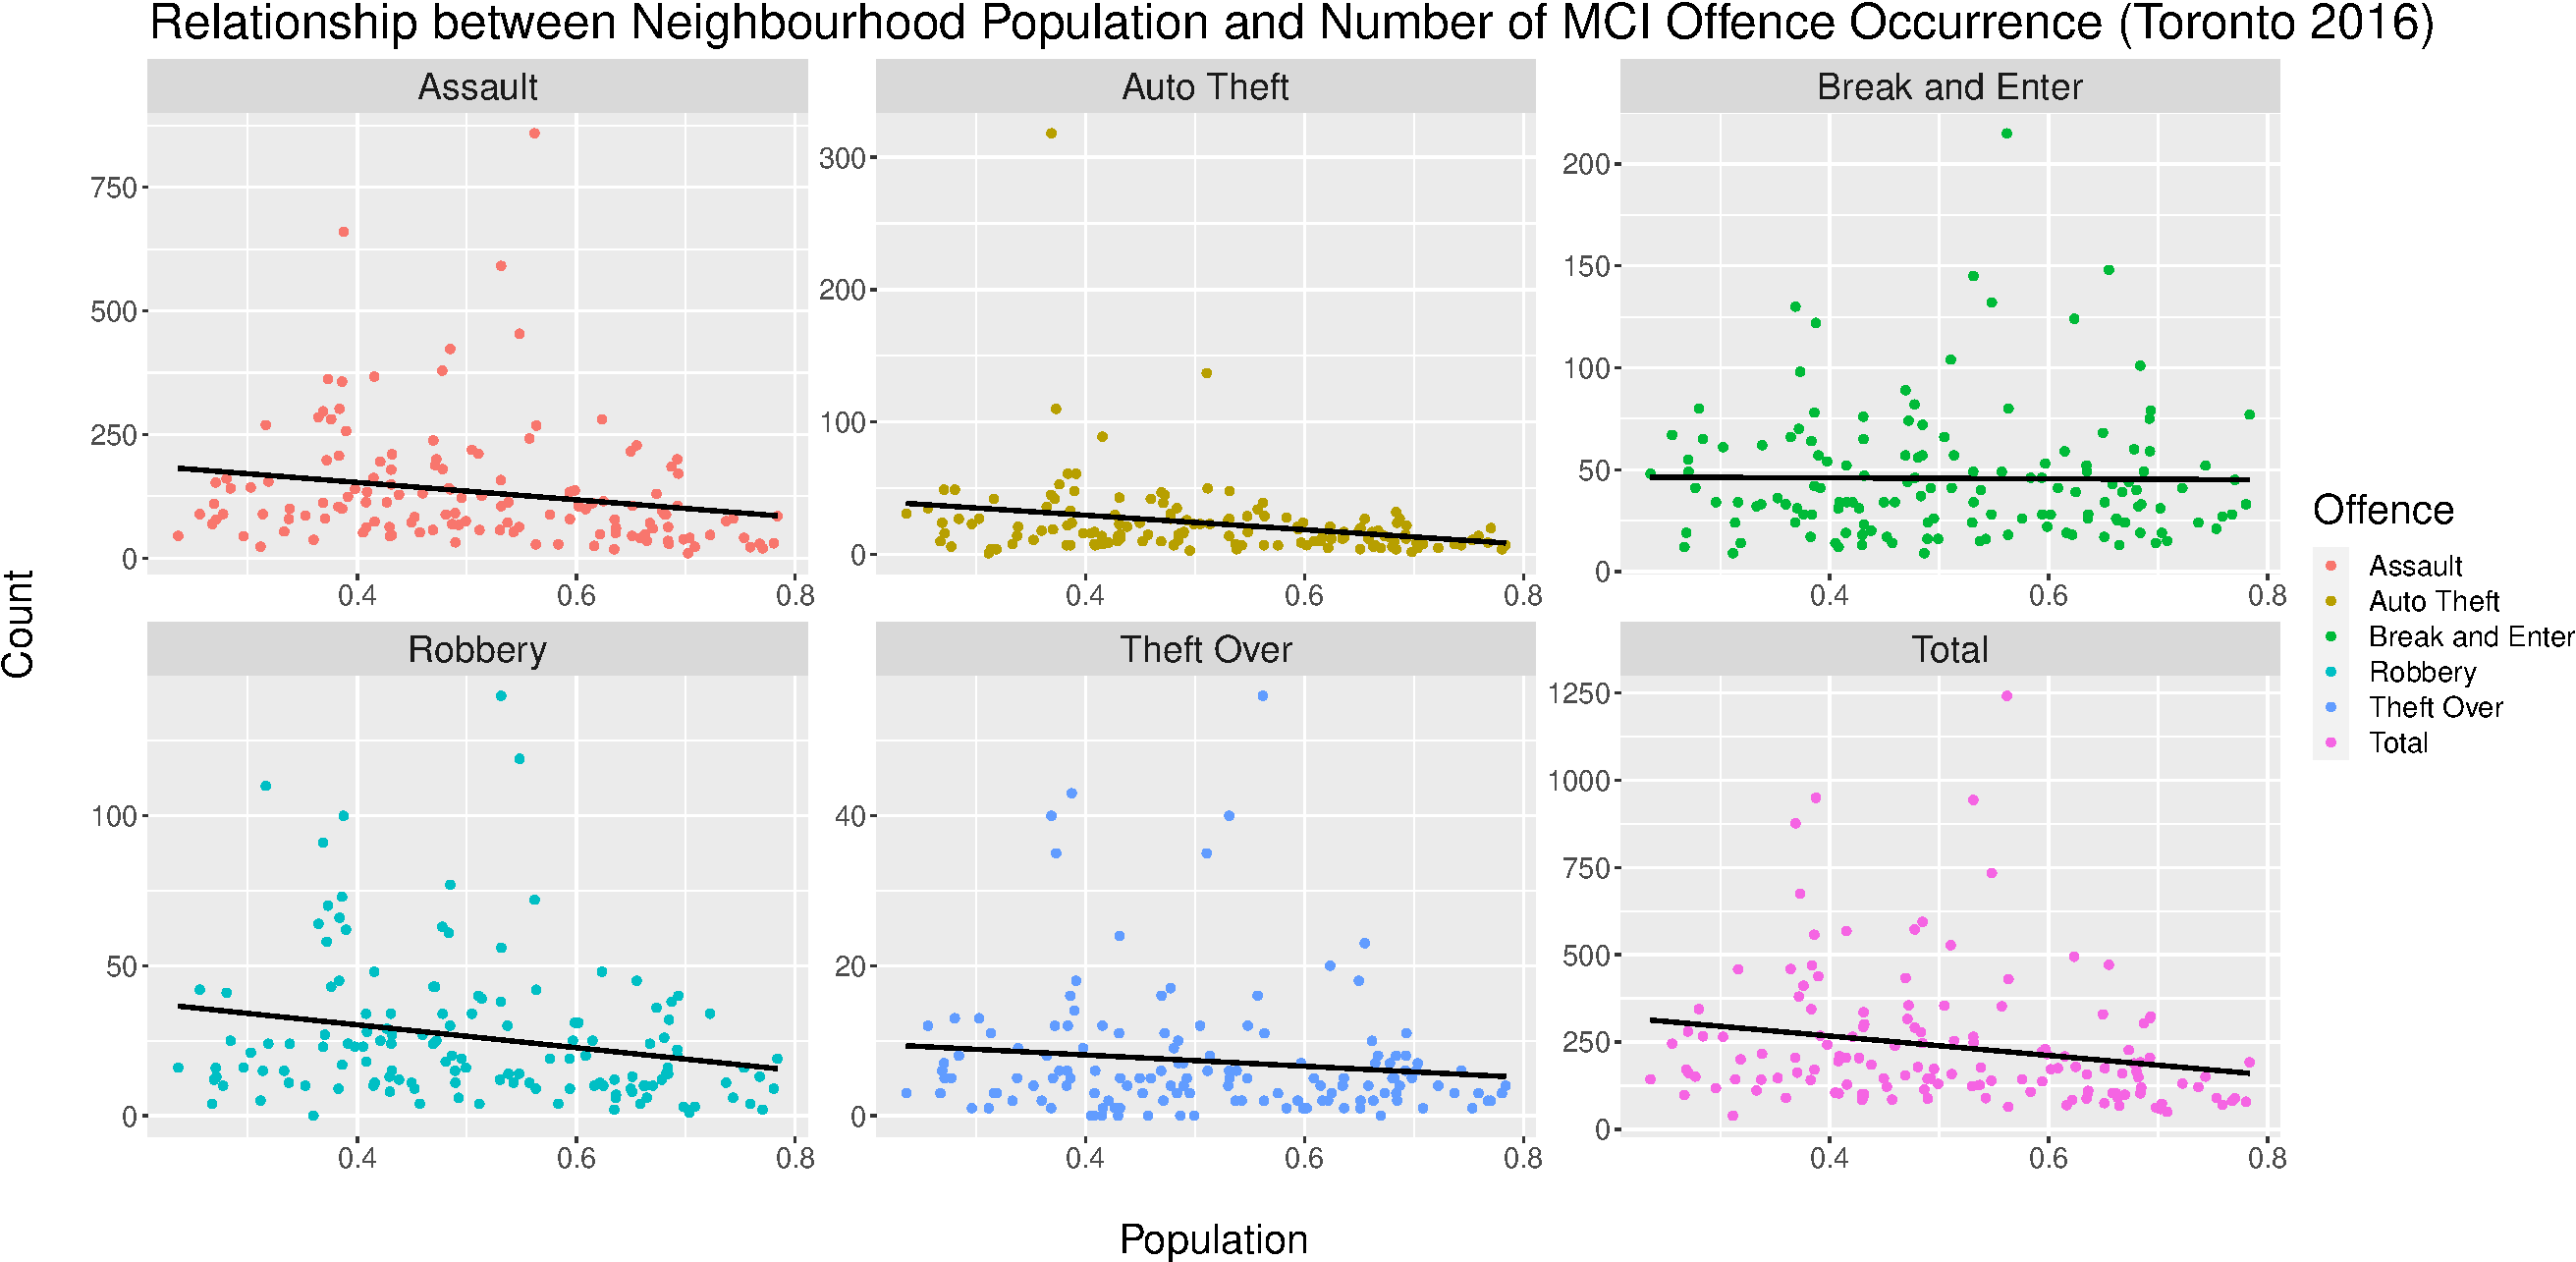
\includegraphics{Final-Report_files/figure-latex/crime-vs-immigration-lm-1.pdf}

\hypertarget{relationship-between-visible-minority-and-crime-rate}{%
\paragraph{2.3.4.6 Relationship between Visible Minority and Crime
Rate}\label{relationship-between-visible-minority-and-crime-rate}}

A racially-diversed neighbourhood were found to be linked to lower crime
rate, especially in rural areas\footnote{Kim, Y.-A., \& Wo, J. C. (2022,
  April 1). Racially diverse neighborhoods in diverse areas are linked
  to lower crime rates. Racially diverse neighborhoods in diverse areas
  are linked to lower crime rates Comments. Retrieved March 13, 2023,
  from
  \url{https://blogs.lse.ac.uk/usappblog/2022/04/01/racially-diverse-neighborhoods-in-diverse-areas-are-linked-to-lower-crime-rates/}}.
Hence, we chose to explore the relationship of neighbourhood crime rate
and the proportion of visible minority because we believed that this
feature was also related to immigration and citizenship status, which
was found to be correlated with crime rate\footnote{Statistics Canada.
  (n.d.). Main article. Neighbourhood Characteristics and the
  Distribution of Police-reported Crime in the City of Toronto.
  Retrieved March 13, 2023, from
  \url{https://www150.statcan.gc.ca/n1/pub/85-561-m/2009018/part-partie1-eng.htm}}.
However, unlike the number of immigrants, we could see that crime rates
were likely to be weakly positively correlated with the proportion of
visible minority in the neighbourhood from the plots. The number of
outliers in the plots might suggest why we obtained a different result
than expected.

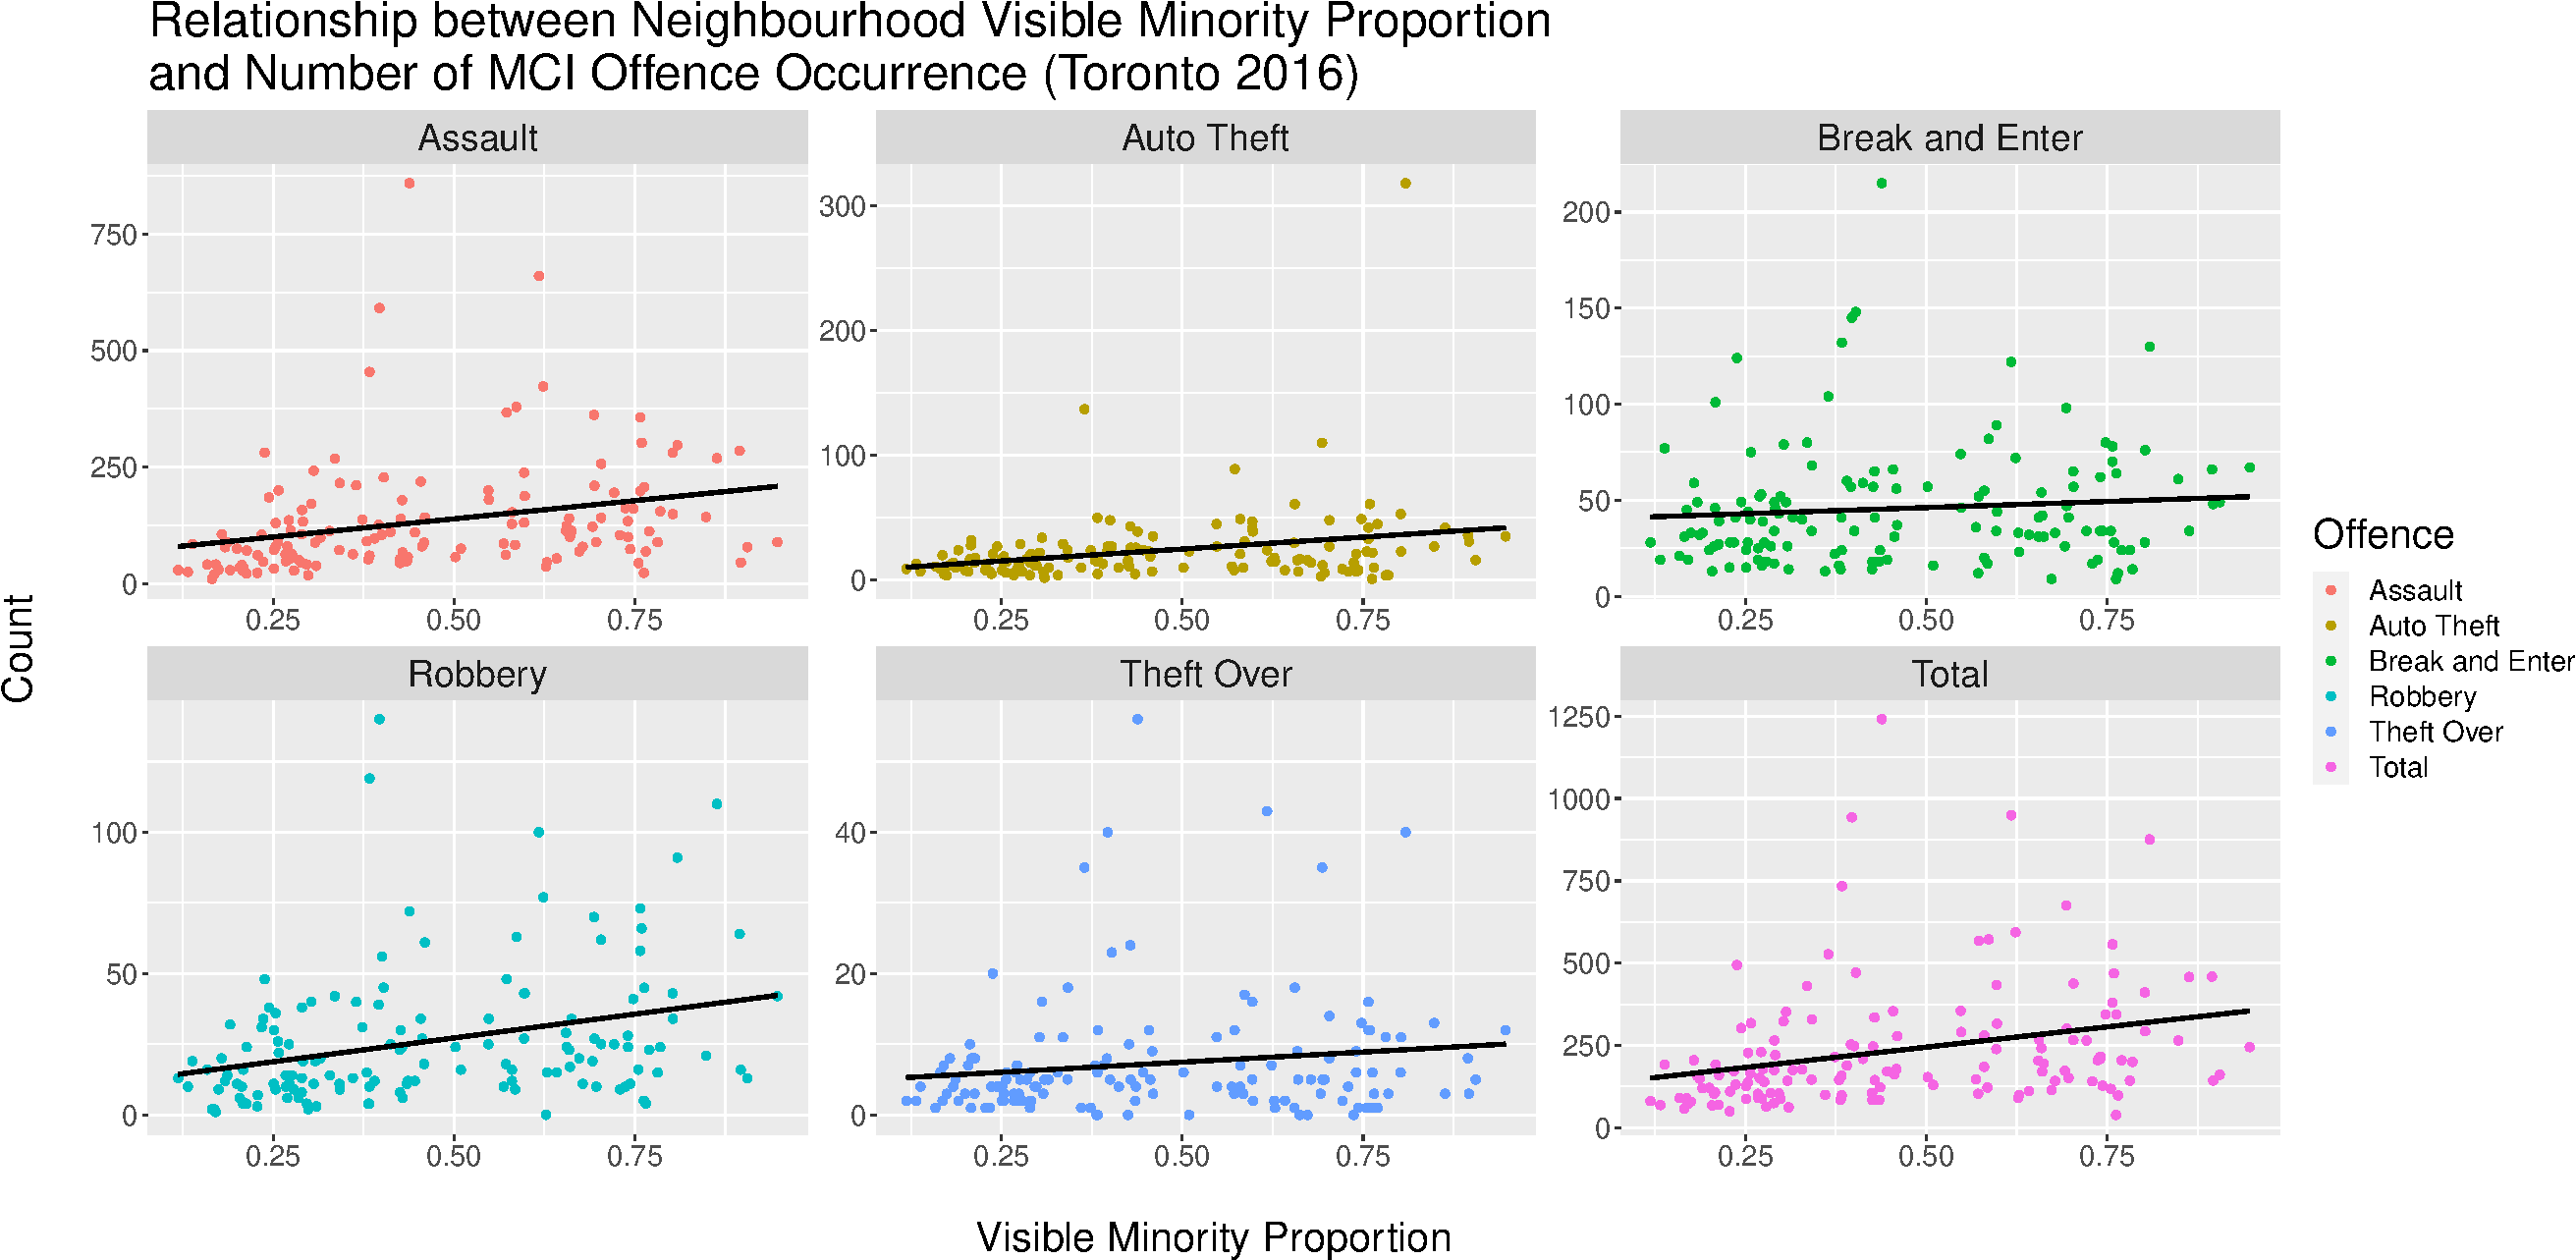
\includegraphics{Final-Report_files/figure-latex/crime-vs-minority-plot-1.pdf}

\hypertarget{relationship-between-income-and-crime-rate}{%
\paragraph{2.3.4.7 Relationship between Income and Crime
Rate}\label{relationship-between-income-and-crime-rate}}

To estimate the effect of average individual income on a neighbourhood's
crime rate, we plotted the number of offences against average income tax
per offence type. The data for income groups were discovered to be
corrupted during data cleaning (see Section 2.2.2). Thus, we used the
average income tax as an indicator of household income level for each
neighbourhood. In the subplots, the numbers of all offence types
decrease as the average income taxes of the neighbourhood increase, with
the exception of ``Break and Enter''. This might be explained by the
fact that wealthy neighbourhoods were more likely to have better
security, and relative risk associated with theft in wealthy
neighbourhoods outweighted the possibility of stealing more expensive
goods, thus deterring thefts\footnote{Chamberlain, A. W., \& Boggess, L.
  N. (2016, September 26). Why disadvantaged neighborhoods are more
  attractive targets for burgling than wealthy ones. Why disadvantaged
  neighborhoods are more attractive targets for burgling than wealthy
  ones Comments. Retrieved March 13, 2023, from
  \url{https://blogs.lse.ac.uk/usappblog/2016/09/26/why-disadvantaged-neighborhoods-are-more-attractive-targets-for-burgling-than-wealthy-ones/}}.

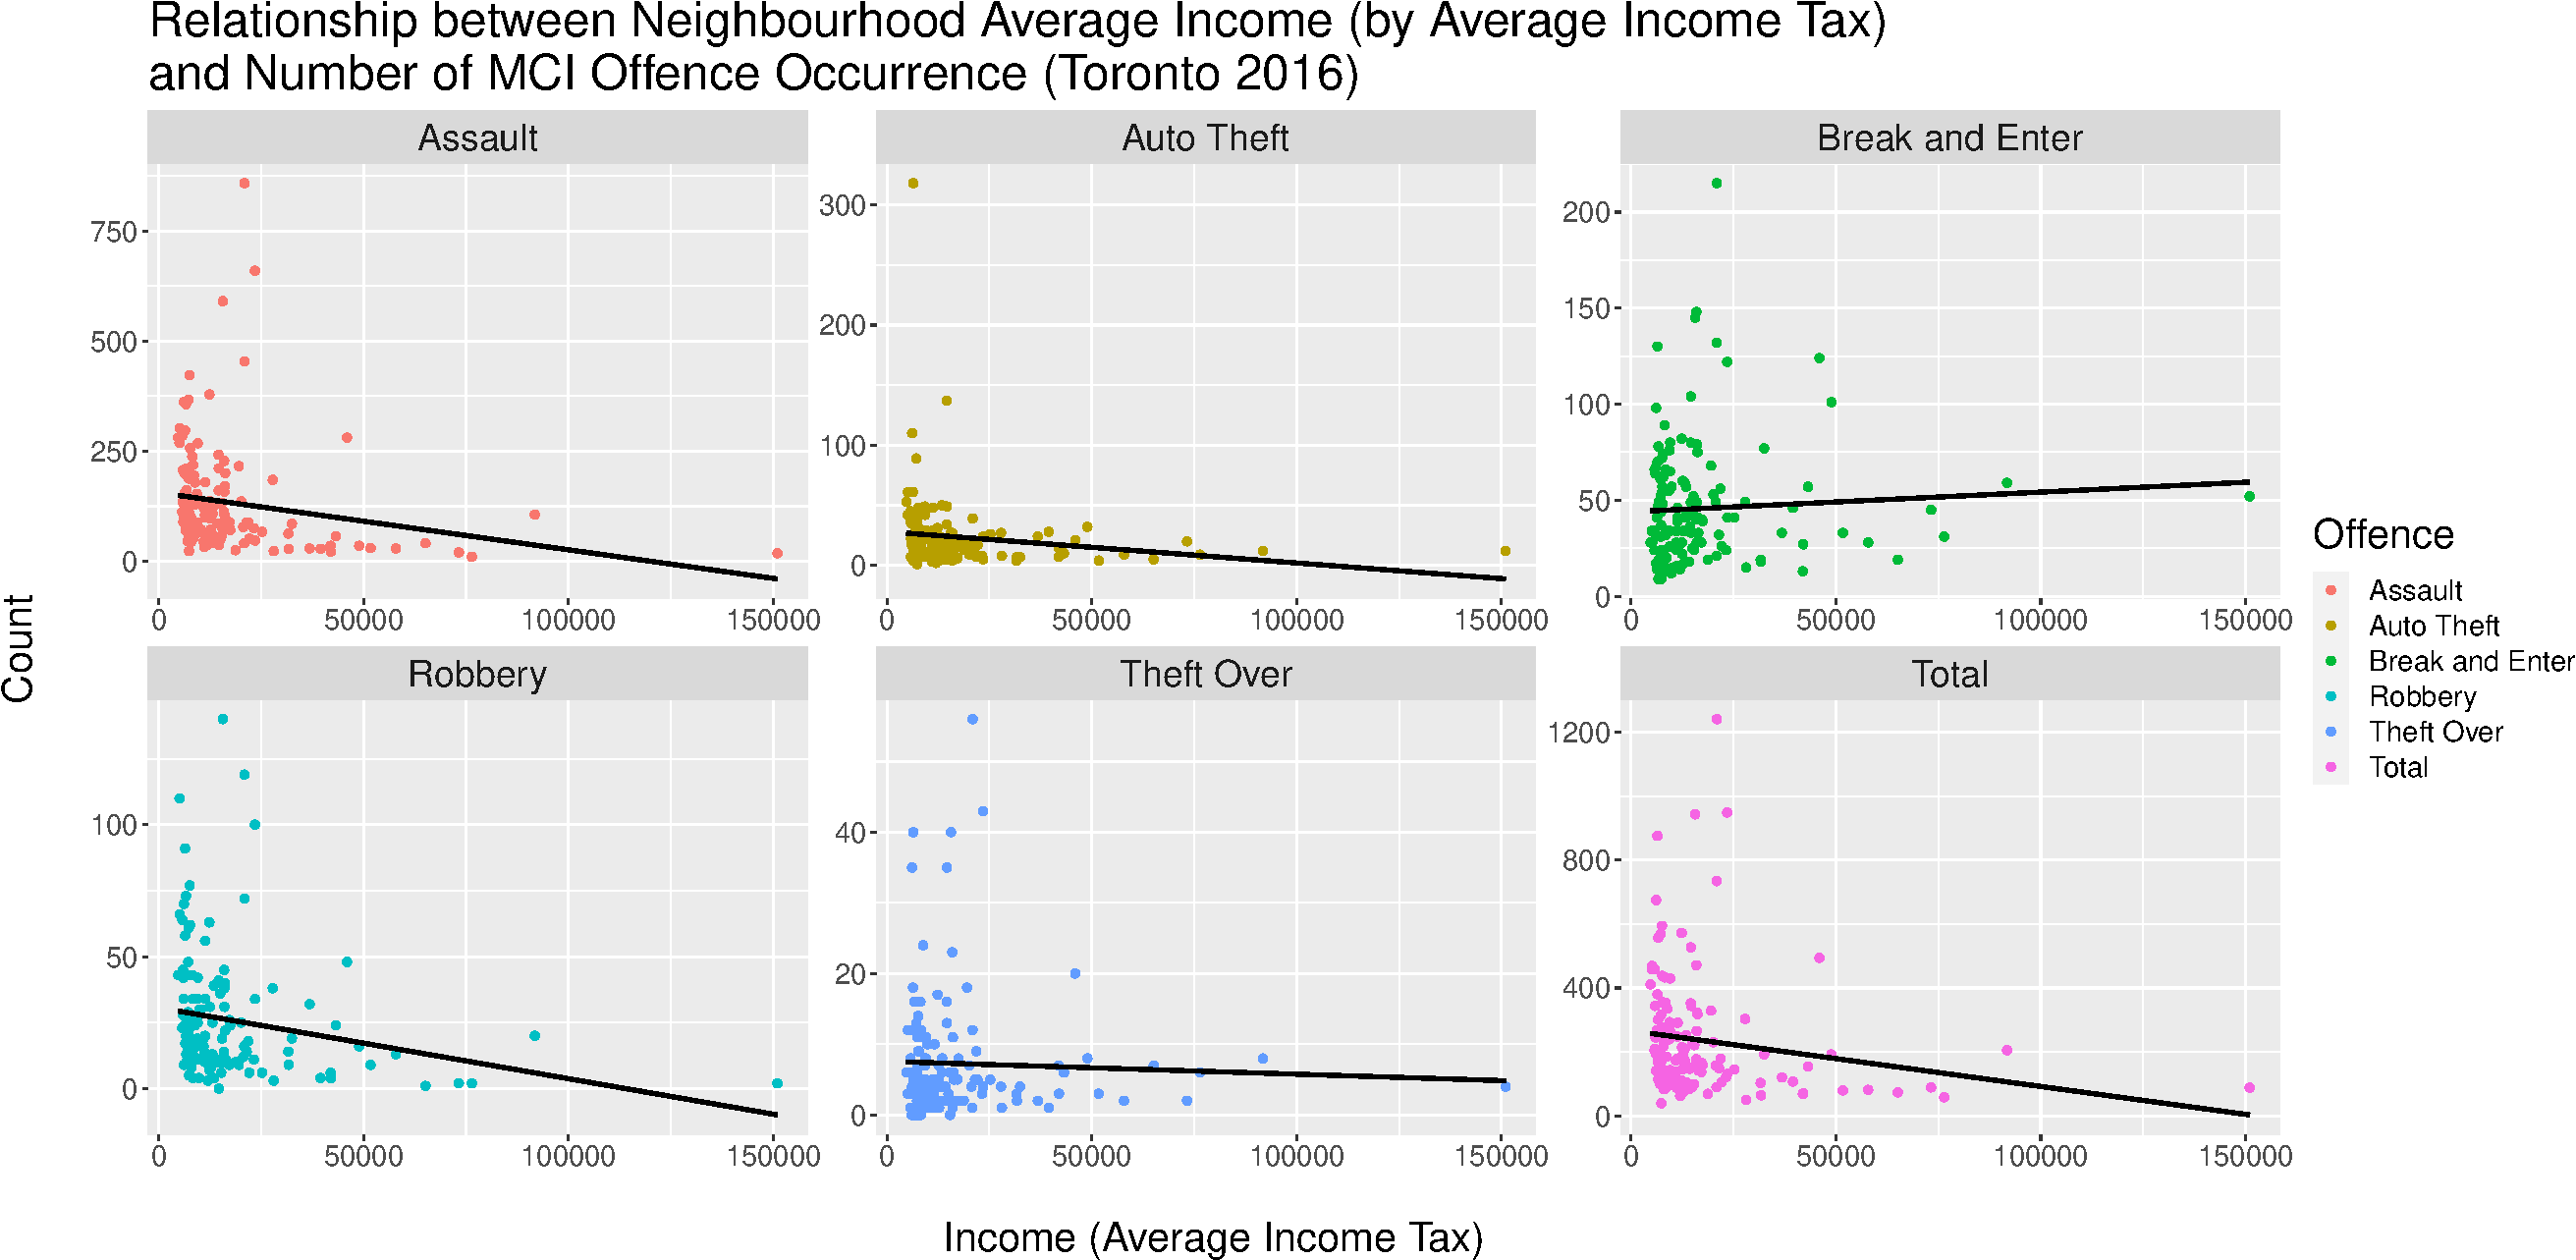
\includegraphics{Final-Report_files/figure-latex/crime-vs-income-plot-1.pdf}

\hypertarget{modelling}{%
\subsection{2.4 Modelling}\label{modelling}}

To investigate which factors have positive effects on crime rate, we
trained several models to predict the number of MCI offences (total
count) using age, level of education, employment status, immigration and
citizenship status, average income tax, number of visible minorities,
and population count, and number of airbnbs, gyms and venues.

The baseline models were Poisson regression model and negative binomial
regression model. The machine learning models trained were regression
tree and random forest.

With only 140 observations corresponding to each neighbourhood, a 80-20
split was used as this ratio gave us enough data for both training and
testing.

A data frame with all variables (response and predictors) of interest
was created using R's merge function, and new variables were created for
regression: for each age group, the ratio between the size of that group
and the size of working age group was created (working age group as
reference); for each education level, the ratio between the number of
people of that level and that of no education was created (non-working
as reference); for each work status, similar ratio was created (ratio
between the number of people working full-time/part-time and that who
did not work); and the proportion of immigrants and visible minority in
each neighbourhood was created.

For Poisson regression and negative binomial regression, a model with
all the predictors was fitted, and the step function was used to perform
backward stepwise regression with Akaike's Information Criterion (AIC)
as the penalty. Afterwards, the variance inflation factors (VIF) were
checked using R's vif function, and variables with VIF greater than 10
were removed and the model was refitted. The final Poisson and negative
binomial models were used as baselines for comparing the performance
against the machine learning models (see below).

A regression tree was fitted using the rpart R library. The complexity
parameter was chosen to be 0 (which resulted in a smaller number of tree
pruning). A variable importance plot was then created to investigate
which factors affect the MCI offence counts to the greatest extents.
Note that all predictors were used in the regression model, whereas in
the Poisson and negative binomial models above, some predictors were
removed due to multicollinearity.

Finally, a random forest was fitted using the randomForest package,
which implemented Breiman's random forest algorithm\footnote{\url{https://www.rdocumentation.org/packages/randomForest/versions/4.7-1.1/topics/randomForest}}.
The number of trees to grow was set to 5000. Similar to the regression
tree model, a variable importance plot was created to interpret which
predictors were the most significant on crime rate.

Although our focus was to investigate which factors affected crime rate
the most, the model performances were evaluated using the
mean-squared-error statistic: each model was used for prediction on both
the training and testing data and the subsequent mean-squared-error for
each data set was calculated. For the basic regression models, the AIC
and the log-likelihood was also calculated for reference.

\hypertarget{results}{%
\section{3. Results}\label{results}}

\hypertarget{poisson-and-negative-binomial-regression}{%
\subsection{3.1 Poisson and Negative Binomial
Regression}\label{poisson-and-negative-binomial-regression}}

The final Poisson regression model fitted was created with all
predictors with the exception of part\_time\_ratio (ratio between number
of people working part time vs not working) and secondary\_ratio (ratio
between number of people with secondary level certificate vs no
education/certificate).

\begin{table}
\begin{wraptable}{l}{0pt}

\caption{\label{tab:poisson-fig}Coefficient Estimates of Poisson Regression Model for Estimating MCI Offence Count}
\centering
\begin{tabular}[t]{l|r|r|r|r}
\hline
Terms & Estimate & Std. Error & t-value & p-value\\
\hline
(Intercept) & 5.659 & 0.080 & 70.971 & 0.000\\
\hline
airbnb & 0.000 & 0.000 & 7.897 & 0.000\\
\hline
gyms & -0.080 & 0.007 & -11.191 & 0.000\\
\hline
venues & 0.001 & 0.000 & 2.186 & 0.029\\
\hline
population & 0.000 & 0.000 & 51.775 & 0.000\\
\hline
children\_ratio & -1.700 & 0.089 & -19.186 & 0.000\\
\hline
youth\_ratio & 4.113 & 0.118 & 34.733 & 0.000\\
\hline
pre\_retirement\_ratio & -2.961 & 0.208 & -14.233 & 0.000\\
\hline
seniors\_ratio & -0.400 & 0.097 & -4.116 & 0.000\\
\hline
postsecondary\_ratio & -0.031 & 0.002 & -16.487 & 0.000\\
\hline
full\_time\_ratio & -0.100 & 0.023 & -4.276 & 0.000\\
\hline
immigrants\_ratio & -0.358 & 0.020 & -18.242 & 0.000\\
\hline
visible\_minority\_ratio & 0.021 & 0.003 & 7.526 & 0.000\\
\hline
\end{tabular}
\end{wraptable}\begin{wraptable}{r}{0pt}

\caption{\label{tab:nb-fig}Coefficient Estimates of Negative Binomial Regression Model for Estimating MCI Offence Count}
\centering
\begin{tabular}[t]{l|r|r|r|r}
\hline
Terms & Estimate & Std. Error & t-value & p-value\\
\hline
(Intercept) & 5.057 & 0.300 & 16.841 & 0.000\\
\hline
gyms & -0.072 & 0.033 & -2.198 & 0.028\\
\hline
venues & 0.003 & 0.002 & 1.768 & 0.077\\
\hline
population & 0.000 & 0.000 & 12.022 & 0.000\\
\hline
children\_ratio & -1.591 & 0.460 & -3.460 & 0.001\\
\hline
youth\_ratio & 3.945 & 0.657 & 6.004 & 0.000\\
\hline
pre\_retirement\_ratio & -2.863 & 0.691 & -4.143 & 0.000\\
\hline
postsecondary\_ratio & -0.042 & 0.010 & -4.057 & 0.000\\
\hline
immigrants\_ratio & -0.253 & 0.077 & -3.265 & 0.001\\
\hline
\end{tabular}
\end{wraptable}
\end{table}

The comparison table above shows the coefficient estimates of the
predictors selected in the fitted Poisson and negative binomial models.
Predictors which appeared in both model had highly similar coefficient
estimates.

In general, age group had the highest impact on the crime rate, as
reflected by the large magnitude of estimated coefficients. The ratio of
visible to non-visible minorities, the number of venues all had a
positive impact on the crime rate. The Poisson model suggested that the
number of Airbnbs in the neighbourhood was not a significant factor of
MCI offence counts. On the other hand, an increase in the number of
gyms, the ratio of people with post-secondary education to one who did
not have any certificates/education, and the ratio of immigrants to
non-immigrants were all linked with a decrease in crime count, with
immigrants playing the most impactful role.

The predictors which was most impactful were the age groups: a one-unit
increase in the ratio of the number of youths (15 - 24 years) to the
number of working age people (25 - 54 years) had a multiplicative impact
of 54 on the mean crime rate (a 53-times increase), while a one-unit
increase in ratio of children (0 - 15 years) and pre-retirement ages (55
- 64 years) was predicted to decrease the mean crime rate by 80\% and
95\% respectively. The p-values of estimated coefficients of the age
group predictors were all very small, which confirmed that the
proportion of different age groups had a statistically significant
impact on MCI offence counts in neighbourhoods.

All predictors in both models, with the exception of the number of
venues in the negative binomial model, were all statistically
significant at the 5\% level.

\begin{longtable}{lrrrr}
\caption*{
{\large Poisson and Negative Binomial Regression Model Statistics}
} \\ 
\toprule
Model & Train.MSE & Test.MSE & AIC & Deviance \\ 
\midrule
Poisson & $9247.67$ & $15630.57$ & $4167.50$ & $3349.88$ \\ 
Negative Binomial & $12793.42$ & $17805.41$ & $1286.32$ & $113.71$ \\ 
\bottomrule
\end{longtable}

The performance of the negative binomial regression model was much
better than the Poission regression model. Although the former model had
higher training and testing MSEs (12793.42 vs Poisson's 9247.67,
17805.41 vs Poisson's 15630.57), it had much lower AIC (1286.32 vs
4167.50) and deviance (113.71 vs 3349.88). Despite their differences,
both models could be adapted as baseline models to evaluate the
performance of the advanced machine learning models.

\hypertarget{regression-tree-and-random-forest}{%
\subsection{3.2 Regression Tree and Random
Forest}\label{regression-tree-and-random-forest}}

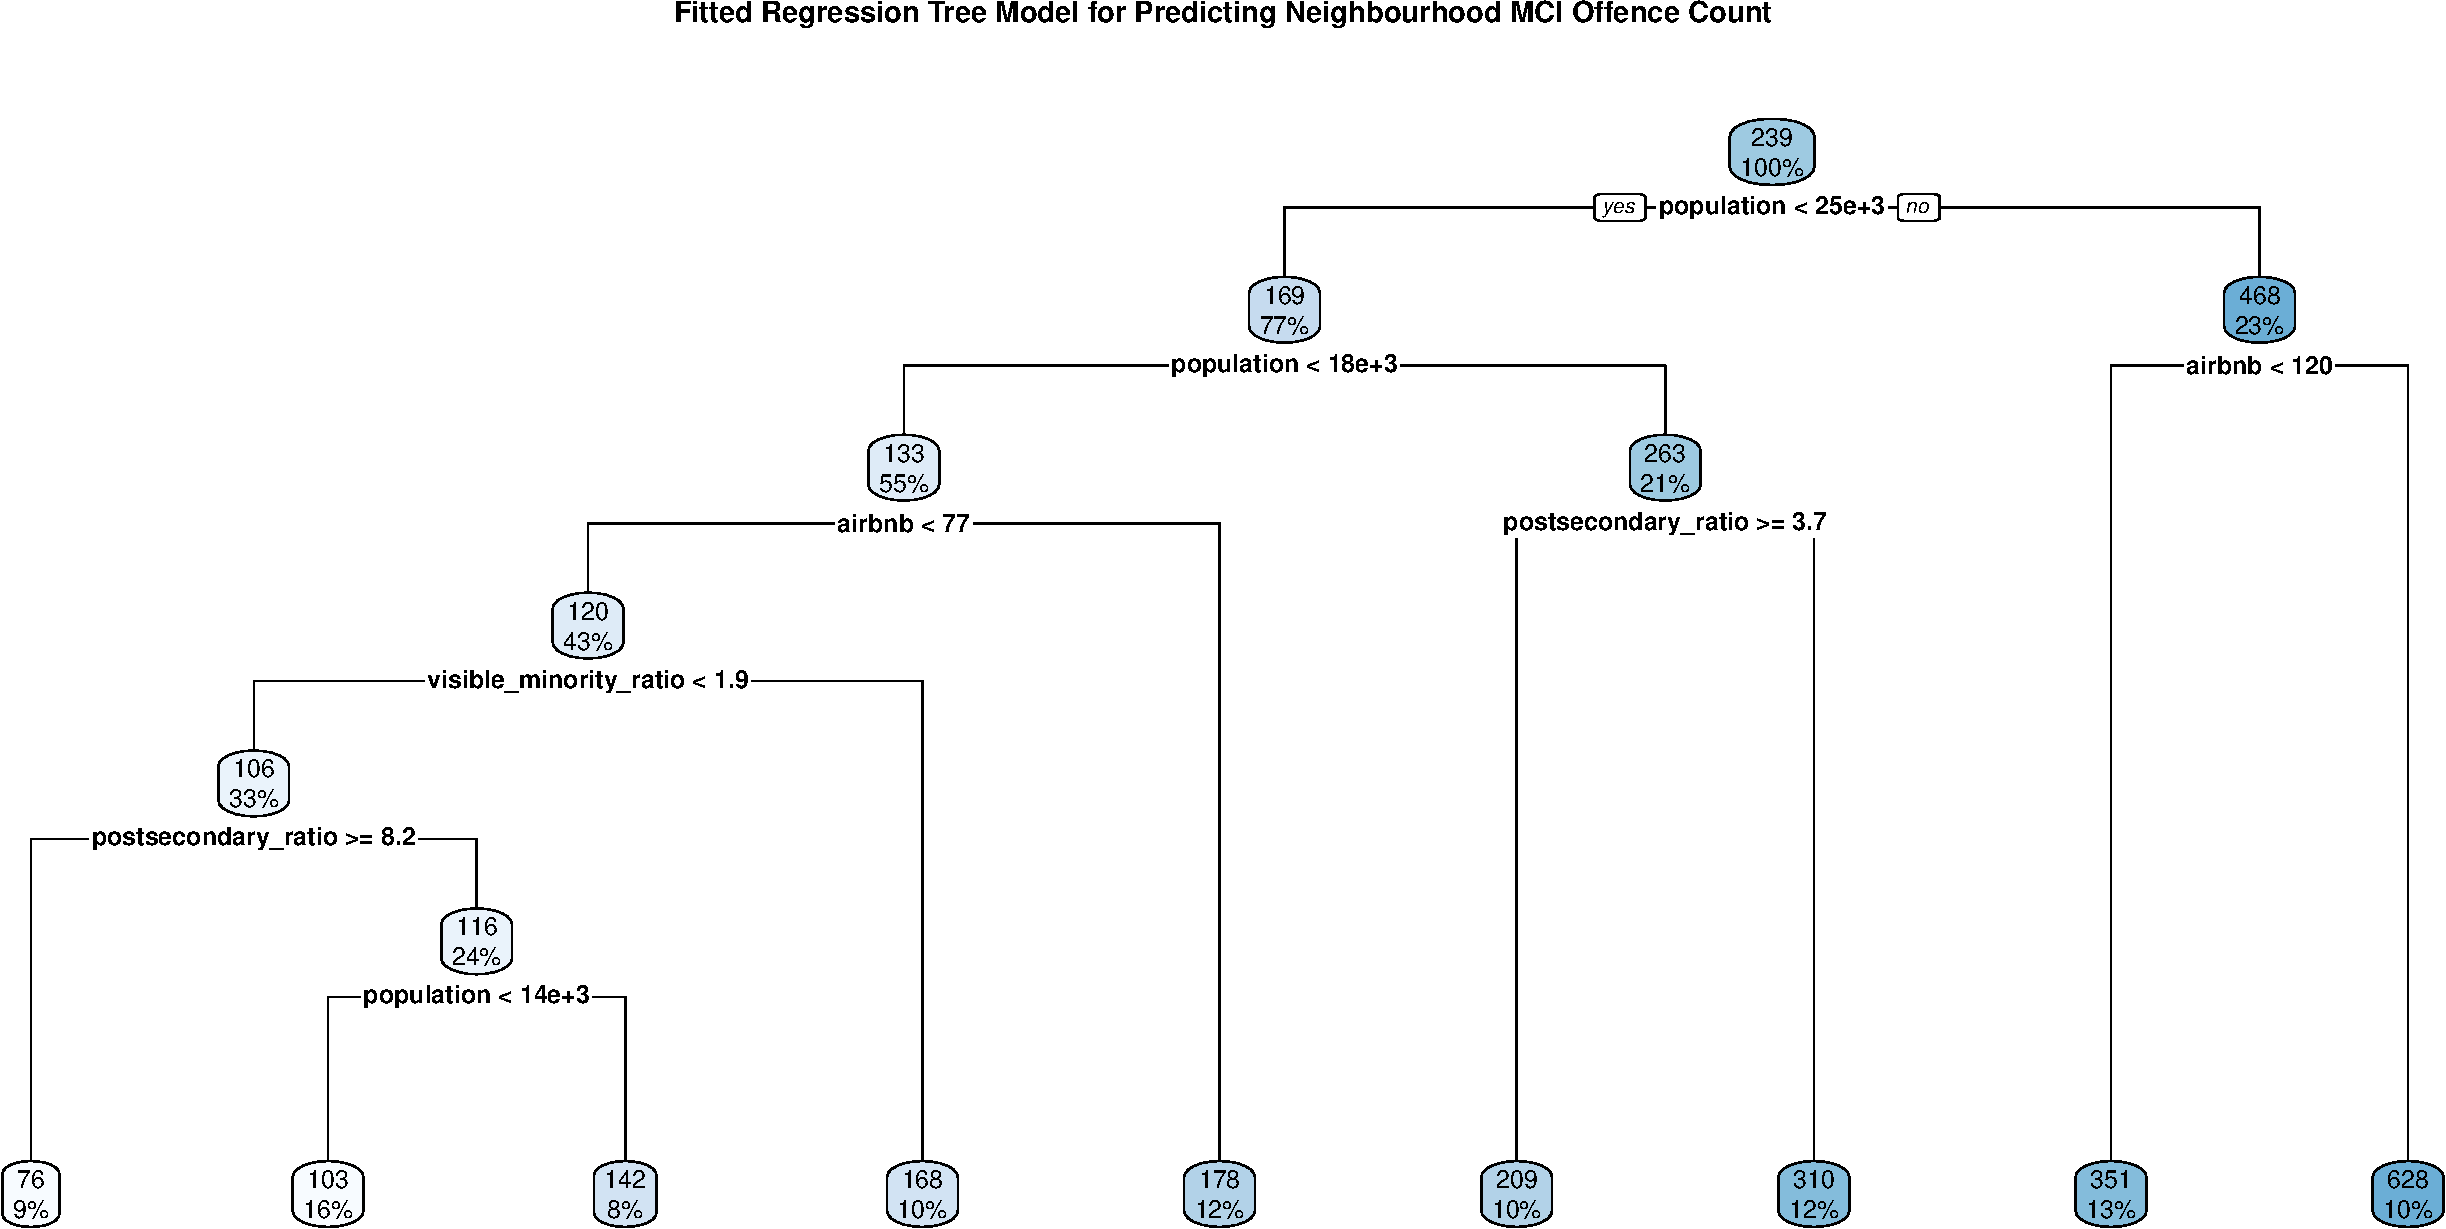
\includegraphics{Final-Report_files/figure-latex/reg-tree-1.pdf}

\begin{longtable}{lrr}
\caption*{
{\large Regression Tree and Random Forest Model Statistics}
} \\ 
\toprule
Model & Train.MSE & Test.MSE \\ 
\midrule
Regression Tree & $15215.15$ & $21061.30$ \\ 
Random Forest & $3113.12$ & $10966.88$ \\ 
\bottomrule
\end{longtable}

The fitted regression tree model with all predictors were simple. The
decision nodes were created by only a few predictors of interest:
population, the number of Airbnbs, the ratio of people with
postsecondary education vs no certificates/education, and the ratio
between visible and non-visible minorities. The resulting tree had only
9 leaves, but the training and test mean-squared-error were both similar
to the baseline regression models. However, the performance of the
random forest was much better than all three model others: it had a
training and test MSE of 3113.12 and 10966.88 respectively.

Despite the simplicity of the regression tree, it may be useful to use
the model as a guideline to predict the MCI offence counts of a
neighbourhood, or as a validation model to validate predictions from
other models.

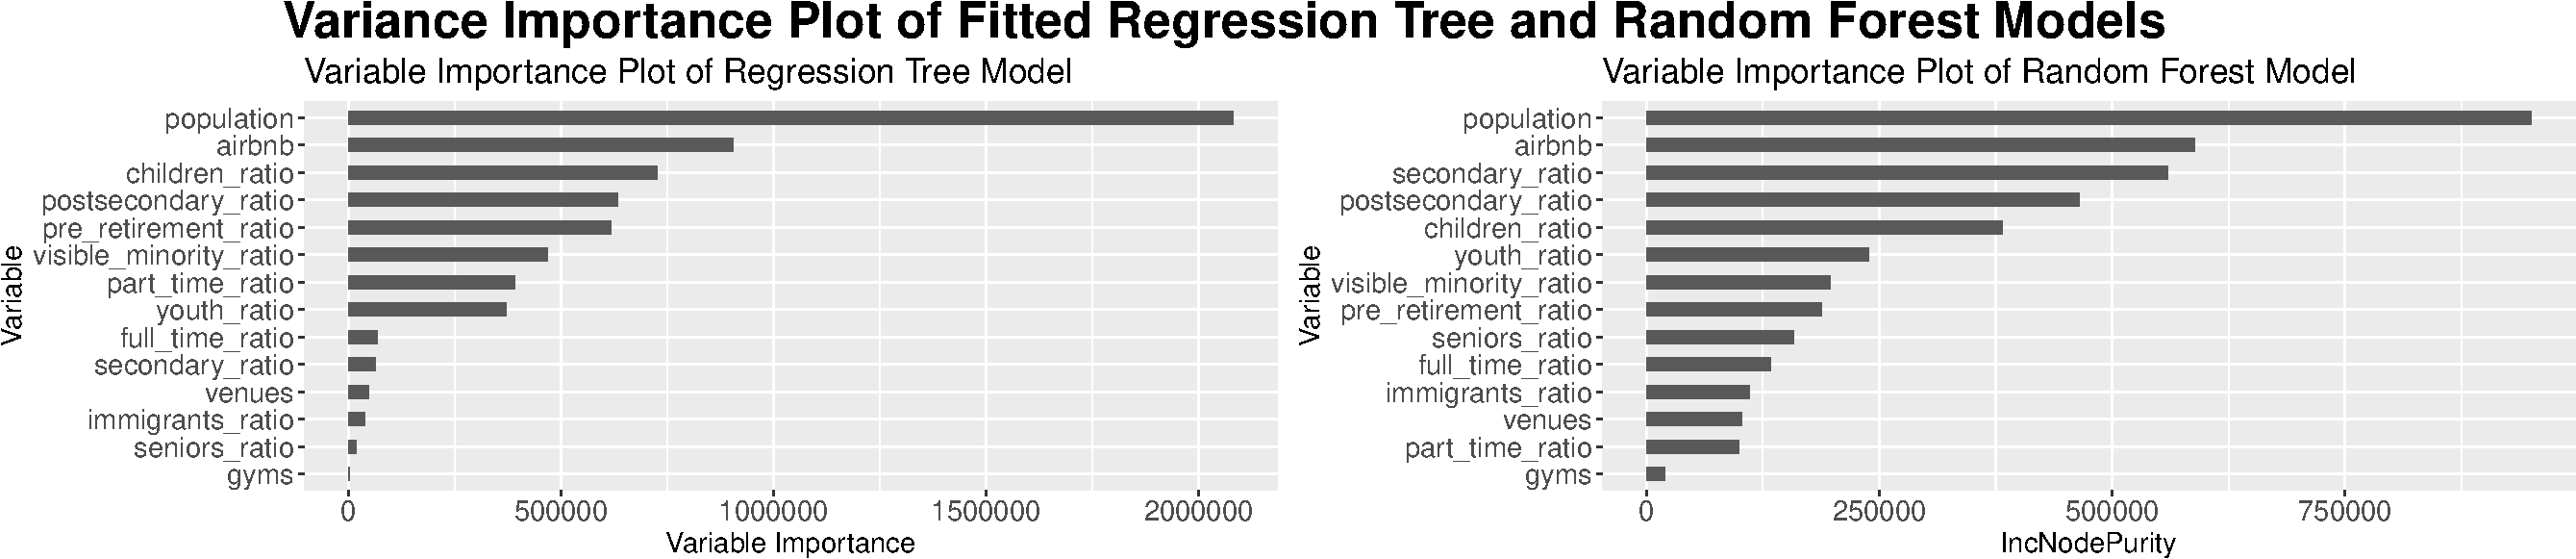
\includegraphics{Final-Report_files/figure-latex/vip-plots-1.pdf}

In general, both the regression tree and random forest suggested that
population and the number of airbnbs were the most important factors of
crime count, followed by education, age and work status (with varying
importance), then immigration and citizenship status, and the number of
venues and gyms had the lowest significance on crime count.

From the variance importance plots, the order of predictors in terms of
variable importance were very similar: population was the most important
factor, which was not surprising as the crime count should be higher for
a larger population. The second most important variable was the number
of Airbnbs, which had the about half of the importance of population.
What followed were education level (ratio between
post-econdary/secondary level education and no certificates), the
proportion (ratio) of children and youths in the neighbourhood, and the
ratio of visible\_minorities vs non-visible minorities. In both models,
the number of venues and gyms were some of the variables with the lowest
importance.

\hypertarget{conclusions-and-summary}{%
\section{4. Conclusions and Summary}\label{conclusions-and-summary}}

In this research study, we aimed to explore the relationship between
Toronto's neighbourhood crime rate and the neighbourhood's demographics
and the community amenities, and investigated which factors affect crime
rate to the greatest extents. Poisson regression, negative binomial
regression, regression tree and random forest models were deployed to
understand this relationship. The fitted random forest model had the
best performance in terms of training and testing mean-squared-error,
followed by Poisson regression, negative binomial regression, and
regression tree.

Our research found out that the population played the largest role on a
neighbourhood's crime rate, followed by different age groups: the
proportion of youths (15 - 24 years) were correlated with the highest
increase in crime, while the proportions of children (0 - 15 years) and
pre-retirement-aged people (55 - 64 years) were correlated with the
largest drop in crime. The proportions of immigrants and visible
minorities were also notable factors of crime, with neigbourhoods of
higher proportion of immigrants and lower visible minorities having
significantly fewer crime occurred. Moreover, people with post-secondary
or secondary education are less likely to commit crime, while an
increase in proportion of people with no certificates or education was
connected to a higher crime rate.

Consistent with previous studies, the number of Airbnb's in the area was
found to be highly correlated with an increase in crime rate. However,
the number of venues (points-of-interests) and gyms did not seem to
affect MCI offences in the area, contrary to prior studies which
concluded that areas with larger business zonings and more tourists
attractions were prone to higher crime rate.

\hypertarget{limitations-and-next-steps}{%
\section{5. Limitations and Next
Steps}\label{limitations-and-next-steps}}

There were several limitations in our research study.

First, the small amount of corrupted/mis-placed observations in the
``Neighbourhood Profiles'' dataset prevented us from using the income
groups directly to estimate the effect of average household and
individual income on neighbourhood crime rate. Instead, we utilised the
average income tax to represent the wealthiness of neighbourhoods.
Although income tax was positively correlated with individual and
household income, the data come in aggregated form (one number,
``average tax income'', for each neighbourhood), compared to the exact
numbers of individuals/household in each household. This reduced the
amount of information we could use and this could affect the final
result in our preliminary testing.

Second, for the regression models, despite the low variance inflation
factors of the predictors, there might be high correlations between
predictors. For example, the proportion of visible minorities in a
neighbourhood might be positively correlated with the number of
immigrants in the area. Although we removed predictors with high VIFs in
the baseline Poisson and negative binomial models, the underlying
relationship between predictors still existed. This limitation was hard
to remove entirely as statistics in demographic data were usually
correlated with one another. In future studies, it might be beneficial
to include a wider variety of data (even if demographic in nature) to
reduce multicollinearity when fitting a regression model.

\hypertarget{references}{%
\section{6. References}\label{references}}

\begin{enumerate}
\def\labelenumi{\arabic{enumi}.}
\item
  Foster, S., Giles-Corti, B., \& Knuiman, M. (2010). Neighbourhood
  design and fear of crime: A social-ecological examination of the
  correlates of residents' fear in new suburban housing developments. In
  Health \& Place (Vol. 16, Issue 6, pp.~1156--1165). Elsevier BV.
  \url{https://doi.org/10.1016/j.healthplace.2010.07.007}
\item
  Statistics Canada. (2021). Neighbourhood characteristics and life
  satisfaction of individuals in lower-, middle-, and higher-income
  families in Canadian metropolitan areas. Government of Canada.
  \url{https://doi.org/10.25318/36280001202100500006-ENG}
\item
  Government of Canada, S. C. (2020, July 17). Census of population.
  Surveys and statistical programs. Retrieved March 13, 2023, from
  \url{https://www23.statcan.gc.ca/imdb/p2SV.pl?Function=getSurvey\&SDDS=3901}
\item
  Statistics Canada. (n.d.). Main article. Neighbourhood Characteristics
  and the Distribution of Police-reported Crime in the City of Toronto.
  Retrieved March 13, 2023, from
  \url{https://www150.statcan.gc.ca/n1/pub/85-561-m/2009018/part-partie1-eng.htm}
\item
  Sun, Ivan Y.; Triplett, Ruth A.; and Gainey, Randy R., ``Neighborhood
  Characteristics and Crime: A Test of Sampson and Groves' Model of
  Social Disorganization'' (2004). Sociology \& Criminal Justice Faculty
  Publications. 3.
  \url{https://digitalcommons.odu.edu/sociology_criminaljustice_fac_pubs/3}
\item
  Ulmer, J. T., \& Steffensmeier, D. (2014). The age and crime
  relationship: Social variation, social explanations. In The Nurture
  Versus Biosocial Debate in Criminology: On the Origins of Criminal
  Behavior and Criminality (pp.~377-396). SAGE Publications Inc..
  \url{https://doi.org/10.4135/9781483349114.n23}
\item
  Farrington, D. P., Gallagher, B., Morley, L., St.~Ledger, R. J., \&
  West, D. J. (1986). UNEMPLOYMENT, SCHOOL LEAVING, AND CRIME. The
  British Journal of Criminology, 26(4), 335--356.
  \url{http://www.jstor.org/stable/23637076}
\item
  Kim, Y.-A., \& Wo, J. C. (2022, April 1). Racially diverse
  neighborhoods in diverse areas are linked to lower crime rates.
  Racially diverse neighborhoods in diverse areas are linked to lower
  crime rates Comments. Retrieved March 13, 2023, from
  \url{https://blogs.lse.ac.uk/usappblog/2022/04/01/racially-diverse-neighborhoods-in-diverse-areas-are-linked-to-lower-crime-rates/}
\item
  Chamberlain, A. W., \& Boggess, L. N. (2016, September 26). Why
  disadvantaged neighborhoods are more attractive targets for burgling
  than wealthy ones. Why disadvantaged neighborhoods are more attractive
  targets for burgling than wealthy ones Comments. Retrieved March 13,
  2023, from
  \url{https://blogs.lse.ac.uk/usappblog/2016/09/26/why-disadvantaged-neighborhoods-are-more-attractive-targets-for-burgling-than-wealthy-ones/}
\item
  Twinam, T. (2017, May 25). Danger zone: Land use and the geography of
  neighborhood crime. Retrieved April 25, 2023, from
  \url{https://www.sciencedirect.com/science/article/abs/pii/S009411901730044X?dgcid=raven_sd_aip_email}
\item
  Ke, L., O'Brien, D. T., \& Heydari, B. (2021, July 14). Airbnb and
  neighborhood crime: The incursion of tourists or the erosion of local
  social dynamics? PLOS ONE. Retrieved April 25, 2023, from
  \url{https://journals.plos.org/plosone/article?id=10.1371\%2Fjournal.pone.0253315}
\end{enumerate}

\hypertarget{appendix}{%
\section{7. Appendix}\label{appendix}}

\hypertarget{table-1.-sample-of-dataset---major-crime-indicators}{%
\subsection{Table 1. Sample of Dataset - Major Crime
Indicators}\label{table-1.-sample-of-dataset---major-crime-indicators}}

\begin{longtable}{rllrrllrrlrlrrlrrlrrlrlrl}
\caption*{
{\large Major Crime Indicators} \\ 
{\small Occurrence of Crime from January 2014 to June 2022}
} \\ 
\toprule
X\_id & event\_unique\_id & Division & occurrencedate & reporteddate & location\_type & premises\_type & ucr\_code & ucr\_ext & offence & reportedyear & reportedmonth & reportedday & reporteddayofyear & reporteddayofweek & reportedhour & occurrenceyear & occurrencemonth & occurrenceday & occurrencedayofyear & occurrencedayofweek & occurrencehour & mci\_category & Hood\_ID & Neighbourhood \\ 
\midrule
1 & GO-20141273318 & D31 & 2014-01-03 & 2014-01-03 & Apartment (Rooming House, Condo) & Apartment & 1430 & 100 & Assault & 2014 & January & 3 & 3 & Friday     & 11 & 2014 & January & 3 & 3 & Friday     & 11 & Assault & 27 & York University Heights \\ 
2 & GO-20141274349 & D42 & 2014-01-03 & 2014-01-03 & Single Home, House (Attach Garage, Cottage, Mobile) & House & 2120 & 200 & B\&E & 2014 & January & 3 & 3 & Friday     & 14 & 2014 & January & 3 & 3 & Friday     & 14 & Break and Enter & 132 & Malvern \\ 
3 & GO-20141274052 & D22 & 2014-01-03 & 2014-01-03 & Open Areas (Lakes, Parks, Rivers) & Outside & 1430 & 100 & Assault & 2014 & January & 3 & 3 & Friday     & 13 & 2014 & January & 3 & 3 & Friday     & 13 & Assault & 19 & Long Branch \\ 
4 & GO-20141276966 & D53 & 2014-01-03 & 2014-01-03 & Other Commercial / Corporate Places (For Profit, Warehouse, Corp. Bldg & Commercial & 2130 & 210 & Theft Over & 2014 & January & 3 & 3 & Friday     & 13 & 2014 & January & 3 & 3 & Friday     & 12 & Theft Over & 55 & Thorncliffe Park \\ 
\bottomrule
\end{longtable}

\hypertarget{table-2.-sample-of-dataset---neighbourhood-profiles-census}{%
\subsection{Table 2. Sample of Dataset - Neighbourhood Profiles
(Census)}\label{table-2.-sample-of-dataset---neighbourhood-profiles-census}}

\begin{longtable}{rllllrllllllllllllllllllllllllllllllllllllllllllllllllllllllllllllllllllllllllllllllllllllllllllllllllllllllllllllllllllllllllllllllllllllllllllll}
\caption*{
{\large Neighbourhood Profiles} \\ 
{\small Census of Neighbourhoods in 2016}
} \\ 
\toprule
X\_id & Category & Topic & Data.Source & Characteristic & City.of.Toronto & Agincourt.North & Agincourt.South.Malvern.West & Alderwood & Annex & Banbury.Don.Mills & Bathurst.Manor & Bay.Street.Corridor & Bayview.Village & Bayview.Woods.Steeles & Bedford.Park.Nortown & Beechborough.Greenbrook & Bendale & Birchcliffe.Cliffside & Black.Creek & Blake.Jones & Briar.Hill.Belgravia & Bridle.Path.Sunnybrook.York.Mills & Broadview.North & Brookhaven.Amesbury & Cabbagetown.South.St..James.Town & Caledonia.Fairbank & Casa.Loma & Centennial.Scarborough & Church.Yonge.Corridor & Clairlea.Birchmount & Clanton.Park & Cliffcrest & Corso.Italia.Davenport & Danforth & Danforth.East.York & Don.Valley.Village & Dorset.Park & Dovercourt.Wallace.Emerson.Junction & Downsview.Roding.CFB & Dufferin.Grove & East.End.Danforth & Edenbridge.Humber.Valley & Eglinton.East & Elms.Old.Rexdale & Englemount.Lawrence & Eringate.Centennial.West.Deane & Etobicoke.West.Mall & Flemingdon.Park & Forest.Hill.North & Forest.Hill.South & Glenfield.Jane.Heights & Greenwood.Coxwell & Guildwood & Henry.Farm & High.Park.North & High.Park.Swansea & Highland.Creek & Hillcrest.Village & Humber.Heights.Westmount & Humber.Summit & Humbermede & Humewood.Cedarvale & Ionview & Islington.City.Centre.West & Junction.Area & Keelesdale.Eglinton.West & Kennedy.Park & Kensington.Chinatown & Kingsview.Village.The.Westway & Kingsway.South & Lambton.Baby.Point & L.Amoreaux & Lansing.Westgate & Lawrence.Park.North & Lawrence.Park.South & Leaside.Bennington & Little.Portugal & Long.Branch & Malvern & Maple.Leaf & Markland.Wood & Milliken & Mimico..includes.Humber.Bay.Shores. & Morningside & Moss.Park & Mount.Dennis & Mount.Olive.Silverstone.Jamestown & Mount.Pleasant.East & Mount.Pleasant.West & New.Toronto & Newtonbrook.East & Newtonbrook.West & Niagara & North.Riverdale & North.St..James.Town & Oakridge & Oakwood.Village & O.Connor.Parkview & Old.East.York & Palmerston.Little.Italy & Parkwoods.Donalda & Pelmo.Park.Humberlea & Playter.Estates.Danforth & Pleasant.View & Princess.Rosethorn & Regent.Park & Rexdale.Kipling & Rockcliffe.Smythe & Roncesvalles & Rosedale.Moore.Park & Rouge & Runnymede.Bloor.West.Village & Rustic & Scarborough.Village & South.Parkdale & South.Riverdale & St.Andrew.Windfields & Steeles & Stonegate.Queensway & Tam.O.Shanter.Sullivan & Taylor.Massey & The.Beaches & Thistletown.Beaumond.Heights & Thorncliffe.Park & Trinity.Bellwoods & University & Victoria.Village & Waterfront.Communities.The.Island & West.Hill & West.Humber.Clairville & Westminster.Branson & Weston & Weston.Pelham.Park & Wexford.Maryvale & Willowdale.East & Willowdale.West & Willowridge.Martingrove.Richview & Woburn & Woodbine.Corridor & Woodbine.Lumsden & Wychwood & Yonge.Eglinton & Yonge.St.Clair & York.University.Heights & Yorkdale.Glen.Park \\ 
\midrule
1 & Neighbourhood Information & Neighbourhood Information & City of Toronto & Neighbourhood Number &  & 129 & 128 & 20 & 95 & 42 & 34 & 76 & 52 & 49 & 39 & 112 & 127 & 122 & 24 & 69 & 108 & 41 & 57 & 30 & 71 & 109 & 96 & 133 & 75 & 120 & 33 & 123 & 92 & 66 & 59 & 47 & 126 & 93 & 26 & 83 & 62 & 9 & 138 & 5 & 32 & 11 & 13 & 44 & 102 & 101 & 25 & 65 & 140 & 53 & 88 & 87 & 134 & 48 & 8 & 21 & 22 & 106 & 125 & 14 & 90 & 110 & 124 & 78 & 6 & 15 & 114 & 117 & 38 & 105 & 103 & 56 & 84 & 19 & 132 & 29 & 12 & 130 & 17 & 135 & 73 & 115 & 2 & 99 & 104 & 18 & 50 & 36 & 82 & 68 & 74 & 121 & 107 & 54 & 58 & 80 & 45 & 23 & 67 & 46 & 10 & 72 & 4 & 111 & 86 & 98 & 131 & 89 & 28 & 139 & 85 & 70 & 40 & 116 & 16 & 118 & 61 & 63 & 3 & 55 & 81 & 79 & 43 & 77 & 136 & 1 & 35 & 113 & 91 & 119 & 51 & 37 & 7 & 137 & 64 & 60 & 94 & 100 & 97 & 27 & 31 \\ 
2 & Neighbourhood Information & Neighbourhood Information & City of Toronto & TSNS2020 Designation &  & No Designation & No Designation & No Designation & No Designation & No Designation & No Designation & No Designation & No Designation & No Designation & No Designation & NIA & No Designation & No Designation & NIA & No Designation & No Designation & No Designation & No Designation & No Designation & No Designation & No Designation & No Designation & No Designation & No Designation & No Designation & No Designation & No Designation & No Designation & No Designation & No Designation & No Designation & Emerging Neighbourhood & No Designation & NIA & No Designation & No Designation & No Designation & NIA & NIA & Emerging Neighbourhood & No Designation & No Designation & NIA & No Designation & No Designation & NIA & No Designation & No Designation & No Designation & No Designation & No Designation & No Designation & No Designation & Emerging Neighbourhood & NIA & NIA & No Designation & NIA & No Designation & No Designation & NIA & NIA & No Designation & NIA & No Designation & No Designation & Emerging Neighbourhood & No Designation & No Designation & No Designation & No Designation & No Designation & No Designation & Emerging Neighbourhood & No Designation & No Designation & No Designation & No Designation & NIA & No Designation & NIA & NIA & No Designation & No Designation & No Designation & No Designation & No Designation & No Designation & No Designation & No Designation & NIA & No Designation & No Designation & No Designation & No Designation & No Designation & No Designation & No Designation & No Designation & No Designation & NIA & No Designation & NIA & No Designation & No Designation & No Designation & No Designation & NIA & NIA & NIA & No Designation & No Designation & Emerging Neighbourhood & No Designation & No Designation & NIA & No Designation & NIA & NIA & No Designation & No Designation & NIA & No Designation & NIA & No Designation & Emerging Neighbourhood & NIA & NIA & No Designation & No Designation & No Designation & No Designation & NIA & No Designation & No Designation & No Designation & No Designation & No Designation & NIA & Emerging Neighbourhood \\ 
3 & Population & Population and dwellings & Census Profile 98-316-X2016001 & Population, 2016 & 2,731,571 & 29,113 & 23,757 & 12,054 & 30,526 & 27,695 & 15,873 & 25,797 & 21,396 & 13,154 & 23,236 & 6,577 & 29,960 & 22,291 & 21,737 & 7,727 & 14,257 & 9,266 & 11,499 & 17,757 & 11,669 & 9,955 & 10,968 & 13,362 & 31,340 & 26,984 & 16,472 & 15,935 & 14,133 & 9,666 & 17,180 & 27,051 & 25,003 & 36,625 & 35,052 & 11,785 & 21,381 & 15,535 & 22,776 & 9,456 & 22,372 & 18,588 & 11,848 & 21,933 & 12,806 & 10,732 & 30,491 & 14,417 & 9,917 & 15,723 & 22,162 & 23,925 & 12,494 & 16,934 & 10,948 & 12,416 & 15,545 & 14,365 & 13,641 & 43,965 & 14,366 & 11,058 & 17,123 & 17,945 & 22,000 & 9,271 & 7,985 & 43,993 & 16,164 & 14,607 & 15,179 & 16,828 & 15,559 & 10,084 & 43,794 & 10,111 & 10,554 & 26,572 & 33,964 & 17,455 & 20,506 & 13,593 & 32,954 & 16,775 & 29,658 & 11,463 & 16,097 & 23,831 & 31,180 & 11,916 & 18,615 & 13,845 & 21,210 & 18,675 & 9,233 & 13,826 & 34,805 & 10,722 & 7,804 & 15,818 & 11,051 & 10,803 & 10,529 & 22,246 & 14,974 & 20,923 & 46,496 & 10,070 & 9,941 & 16,724 & 21,849 & 27,876 & 17,812 & 24,623 & 25,051 & 27,446 & 15,683 & 21,567 & 10,360 & 21,108 & 16,556 & 7,607 & 17,510 & 65,913 & 27,392 & 33,312 & 26,274 & 17,992 & 11,098 & 27,917 & 50,434 & 16,936 & 22,156 & 53,485 & 12,541 & 7,865 & 14,349 & 11,817 & 12,528 & 27,593 & 14,804 \\ 
4 & Population & Population and dwellings & Census Profile 98-316-X2016001 & Population, 2011 & 2,615,060 & 30,279 & 21,988 & 11,904 & 29,177 & 26,918 & 15,434 & 19,348 & 17,671 & 13,530 & 23,185 & 6,488 & 27,876 & 21,856 & 22,057 & 7,763 & 14,302 & 8,713 & 11,563 & 17,787 & 12,053 & 9,851 & 10,487 & 13,093 & 28,349 & 24,770 & 14,612 & 15,703 & 13,743 & 9,444 & 16,712 & 26,739 & 24,363 & 34,631 & 34,659 & 11,449 & 20,839 & 14,943 & 22,829 & 9,550 & 22,086 & 18,810 & 10,927 & 22,168 & 12,474 & 10,926 & 31,390 & 14,083 & 9,816 & 11,333 & 21,292 & 21,740 & 13,097 & 17,656 & 10,583 & 12,525 & 15,853 & 14,108 & 13,091 & 38,084 & 14,027 & 10,638 & 17,058 & 18,495 & 21,723 & 9,170 & 7,921 & 44,919 & 14,642 & 14,541 & 15,070 & 17,011 & 12,050 & 9,632 & 45,086 & 10,197 & 10,436 & 27,167 & 26,541 & 17,587 & 16,306 & 13,145 & 32,788 & 15,982 & 28,593 & 10,900 & 16,423 & 23,052 & 21,274 & 12,191 & 17,832 & 13,497 & 21,073 & 18,316 & 9,118 & 13,746 & 34,617 & 8,710 & 7,653 & 16,144 & 11,197 & 10,007 & 10,488 & 22,267 & 15,050 & 20,631 & 45,912 & 9,632 & 9,951 & 16,609 & 21,251 & 25,642 & 17,958 & 25,017 & 24,691 & 27,398 & 15,594 & 21,130 & 10,138 & 19,225 & 16,802 & 7,782 & 17,182 & 43,361 & 26,547 & 34,100 & 25,446 & 18,170 & 12,010 & 27,018 & 45,041 & 15,004 & 21,343 & 53,350 & 11,703 & 7,826 & 13,986 & 10,578 & 11,652 & 27,713 & 14,687 \\ 
\bottomrule
\end{longtable}

\hypertarget{table-3.-sample-of-dataset---airbnb-toronto-data}{%
\subsection{Table 3. Sample of Dataset - Airbnb Toronto
Data}\label{table-3.-sample-of-dataset---airbnb-toronto-data}}

\begin{longtable}{rllllllrrrlrrrrrlr}
\caption*{
{\large Airbnb Toronto Data} \\ 
{\small Airbnb Listings in Toronto 2016}
} \\ 
\toprule
id & listing\_url & host\_name & neighbourhood & neighbourhood\_cleansed & property\_type & room\_type & price & minimum\_nights & maximum\_nights & has\_availability & availability\_30 & availability\_60 & availability\_90 & availability\_365 & number\_of\_reviews & license & calculated\_host\_listings\_count \\ 
\midrule
27640141 & https://www.airbnb.com/rooms/27640141 & Liora & Toronto & Dovercourt-Wallace Emerson-Junction & Entire guest suite & Entire home/apt & 90 & 28 & 1125 & t & 0 & 25 & 55 & 145 & 47 & Unlicensed & 2 \\ 
27826009 & https://www.airbnb.com/rooms/27826009 & Brianne & Toronto & Waterfront Communities-The Island & Entire condo & Entire home/apt & 130 & 28 & 1125 & t & 0 & 0 & 0 & 0 & 2 & Unlicensed & 1 \\ 
27647117 & https://www.airbnb.com/rooms/27647117 & Alexandra & Toronto & Playter Estates-Danforth & Entire rental unit & Entire home/apt & 45 & 28 & 30 & t & 0 & 0 & 0 & 0 & 4 & Unlicensed & 1 \\ 
27647509 & https://www.airbnb.com/rooms/27647509 & Rosana & Toronto & High Park North & Private room in rental unit & Private room & 80 & 28 & 1125 & t & 0 & 0 & 0 & 0 & 9 & Unlicensed & 1 \\ 
\bottomrule
\end{longtable}

\hypertarget{table-4.-sample-of-dataset---toronto-neighbourhoods-information}{%
\subsection{Table 4. Sample of Dataset - Toronto Neighbourhoods
Information}\label{table-4.-sample-of-dataset---toronto-neighbourhoods-information}}

\begin{longtable}{lrrrrlrr}
\caption*{
{\large Toronto Neighbourhoods Information}
} \\ 
\toprule
Neighborhood & Total.population & number.of.educated.people & number.of.15.45 & number.of.employers & long\_latt & number\_gyms & number\_venues \\ 
\midrule
Agincourt North & 30280 & 19805 & 11850 & 13230 & [-79.2816161258827, 43.797405754163] & 0 & 26 \\ 
Agincourt South-Malvern West & 21990 & 14535 & 8840 & 9860 & [-79.2891688527481, 43.7851873380096] & 0 & 34 \\ 
Alderwood & 11900 & 7915 & 4520 & 6240 & [-79.5532040267975, 43.5954996876866] & 1 & 17 \\ 
Annex & 29180 & 23495 & 15095 & 16770 & [-79.4121466573202, 43.6744312990078] & 3 & 63 \\ 
\bottomrule
\end{longtable}

\hypertarget{table-5.-sample-of-cleaned-dataset---major-crime-indicators}{%
\subsection{Table 5. Sample of Cleaned Dataset - Major Crime
Indicators}\label{table-5.-sample-of-cleaned-dataset---major-crime-indicators}}

\begin{longtable}{rrlllrlrrlrrlrrlrlrl}
\caption*{
{\large Major Crime Indicators (2016)} \\ 
{\small Occurrence of Crime in 2016}
} \\ 
\toprule
occurrencedate & reporteddate & location\_type & premises\_type & offence & reportedyear & reportedmonth & reportedday & reporteddayofyear & reporteddayofweek & reportedhour & occurrenceyear & occurrencemonth & occurrenceday & occurrencedayofyear & occurrencedayofweek & occurrencehour & mci\_category & Hood\_ID & Neighbourhood \\ 
\midrule
2016-01-01 & 2016-01-01 & Apartment (Rooming House, Condo) & Apartment & Assault With Weapon & 2016 & January & 1 & 1 & Friday     & 3 & 2016 & January & 1 & 1 & Friday     & 3 & Assault & 70 & South Riverdale \\ 
2016-01-06 & 2016-01-06 & Single Home, House (Attach Garage, Cottage, Mobile) & House & B\&E & 2016 & January & 6 & 6 & Wednesday  & 13 & 2016 & January & 6 & 6 & Wednesday  & 13 & Break and Enter & 86 & Roncesvalles \\ 
2016-01-01 & 2016-01-01 & Single Home, House (Attach Garage, Cottage, Mobile) & House & Assault With Weapon & 2016 & January & 1 & 1 & Friday     & 4 & 2016 & January & 1 & 1 & Friday     & 3 & Assault & 31 & Yorkdale-Glen Park \\ 
2016-01-06 & 2016-01-06 & Streets, Roads, Highways (Bicycle Path, Private Road) & Outside & Robbery - Mugging & 2016 & January & 6 & 6 & Wednesday  & 12 & 2016 & January & 6 & 6 & Wednesday  & 12 & Robbery & 101 & Forest Hill South \\ 
\bottomrule
\end{longtable}

\hypertarget{table-6.-sample-of-cleaned-dataset---airbnb-toronto-data}{%
\subsection{Table 6. Sample of Cleaned Dataset - Airbnb Toronto
Data}\label{table-6.-sample-of-cleaned-dataset---airbnb-toronto-data}}

\begin{longtable}{rllllllrrrlrrrrrlr}
\caption*{
{\large Airbnb Toronto Data}
} \\ 
\toprule
id & listing\_url & host\_name & neighbourhood & neighbourhood\_cleansed & property\_type & room\_type & price & minimum\_nights & maximum\_nights & has\_availability & availability\_30 & availability\_60 & availability\_90 & availability\_365 & number\_of\_reviews & license & calculated\_host\_listings\_count \\ 
\midrule
27640141 & https://www.airbnb.com/rooms/27640141 & Liora & Toronto & Dovercourt Wallace Emerson Junction & Entire guest suite & Entire home/apt & 90 & 28 & 1125 & t & 0 & 25 & 55 & 145 & 47 & Unlicensed & 2 \\ 
27826009 & https://www.airbnb.com/rooms/27826009 & Brianne & Toronto & Waterfront Communities The Island & Entire condo & Entire home/apt & 130 & 28 & 1125 & t & 0 & 0 & 0 & 0 & 2 & Unlicensed & 1 \\ 
27647117 & https://www.airbnb.com/rooms/27647117 & Alexandra & Toronto & Playter Estates Danforth & Entire rental unit & Entire home/apt & 45 & 28 & 30 & t & 0 & 0 & 0 & 0 & 4 & Unlicensed & 1 \\ 
27647509 & https://www.airbnb.com/rooms/27647509 & Rosana & Toronto & High Park North & Private room in rental unit & Private room & 80 & 28 & 1125 & t & 0 & 0 & 0 & 0 & 9 & Unlicensed & 1 \\ 
\bottomrule
\end{longtable}

\hypertarget{table-7.-sample-of-cleaned-dataset---toronto-neighbourhoods-information}{%
\subsection{Table 7. Sample of Cleaned Dataset - Toronto Neighbourhoods
Information}\label{table-7.-sample-of-cleaned-dataset---toronto-neighbourhoods-information}}

\begin{longtable}{lrr}
\caption*{
{\large Airbnb Toronto Data}
} \\ 
\toprule
Neighbourhood & number\_gyms & number\_venues \\ 
\midrule
Agincourt North & 0 & 26 \\ 
Agincourt South Malvern West & 0 & 34 \\ 
Alderwood & 1 & 17 \\ 
Annex & 3 & 63 \\ 
Banbury Don Mills & 2 & 14 \\ 
Bathurst Manor & 1 & 26 \\ 
Bay Street Corridor & 1 & 96 \\ 
Bayview Village & 3 & 37 \\ 
\bottomrule
\end{longtable}

\end{document}
